%%%%%%%%%%%%%%%%%%%%%%%%%%%%%%%%%%%%%%%%%
% Beamer Presentation
% LaTeX Template
% Version 1.0 (10/11/12)
%
% This template has been downloaded from:
% http://www.LaTeXTemplates.com
%
% License:
% CC BY-NC-SA 3.0 (http://creativecommons.org/licenses/by-nc-sa/3.0/)
%
%%%%%%%%%%%%%%%%%%%%%%%%%%%%%%%%%%%%%%%%%

%----------------------------------------------------------------------------------------
%	PACKAGES AND THEMES
%----------------------------------------------------------------------------------------

\documentclass{beamer}

\mode<presentation> {

% The Beamer class comes with a number of default slide themes
% which change the colors and layouts of slides. Below this is a list
% of all the themes, uncomment each in turn to see what they look like.

%\usetheme{default}
%\usetheme{AnnArbor}
%\usetheme{Antibes}
%\usetheme{Bergen}
%\usetheme{Berkeley}
%\usetheme{Berlin}
%\usetheme{Boadilla}
%\usetheme{CambridgeUS}
%\usetheme{Copenhagen}
%\usetheme{Darmstadt}
%\usetheme{Dresden}
%\usetheme{Frankfurt}
%\usetheme{Goettingen}
%\usetheme{Hannover}
%\usetheme{Ilmenau}
%\usetheme{JuanLesPins}
%\usetheme{Luebeck}
\usetheme{Madrid}
%\usetheme{Malmoe}
%\usetheme{Marburg}
%\usetheme{Montpellier}
%\usetheme{PaloAlto}
%\usetheme{Pittsburgh}
%\usetheme{Rochester}
%\usetheme{Singapore}
%\usetheme{Szeged}
%\usetheme{Warsaw}

% As well as themes, the Beamer class has a number of color themes
% for any slide theme. Uncomment each of these in turn to see how it
% changes the colors of your current slide theme.

%\usecolortheme{albatross}
%\usecolortheme{beaver}
%\usecolortheme{beetle}
%\usecolortheme{crane}
%\usecolortheme{dolphin}
%\usecolortheme{dove}
%\usecolortheme{fly}
%\usecolortheme{lily}
%\usecolortheme{orchid}
%\usecolortheme{rose}
%\usecolortheme{seagull}
%\usecolortheme{seahorse}
%\usecolortheme{whale}
%\usecolortheme{wolverine}

%\setbeamertemplate{footline} % To remove the footer line in all slides uncomment this line
%\setbeamertemplate{footline}[page number] % To replace the footer line in all slides with a simple slide count uncomment this line

\setbeamertemplate{navigation symbols}{} % To remove the navigation symbols from the bottom of all slides uncomment this line
}

\usepackage{graphicx} % Allows including images
%\usepackage{booktabs} % Allows the use of \toprule, \midrule and
                      % \bottomrule in tables
\usepackage{tikz}
\usepackage{pgfplots}
\usepackage{tikz-cd}
\usepackage{bm}
\usepackage{mathtools}
\usepackage{varwidth}
\usepackage{amsmath}
\usepackage[author-year]{amsrefs}
\usepackage{../ReAdTeX/readtex-core}
% \usepackage{../ReAdTeX/readtex-dangerous}
% \usepackage{../ReAdTeX/readtex-abstract-algebra}
\usepackage{ytableau}
\usepackage{hyperref}
%%%%%%%%%%%%%%%%%%%%%%%%%%%%%%%%%%%%%%%%%%%%%%%%%%%%%%%%%%%%%%%%%%% 
%%  MACRO DEFINITIONS:  Co-authors -- PLEASE use these! 
%%%%%%%%%%%%%%%%%%%%%%%%%%%%%%%%%%%%%%%%%%%%%%%%%%%%%%%%%%%%%%%%%%%
\definecolor{coralred}{rgb}{1.0, 0.25, 0.25}
\definecolor{lightblue}{rgb}{.3,.65,1.0} %
\DeclareMathOperator{\Gr}{Gr}
\newcommand{\cupprod}{\cup}
\newcommand{\sym}{\Lambda}
\newcommand{\lowers}{\mathcal{L}}
\newcommand{\mynone}{\ }
\newcommand{\G}{\mathfrak{G}}
\renewcommand{\S}{\mathfrak{S}}
\DeclareMathOperator{\SSYT}{SSYT}
\renewcommand{\Span}{\operatorname{sp}}
\DeclareMathOperator{\area}{area}
\DeclareMathOperator{\dinv}{dinv}
\newcommand{\DP}{\mathbf{DP}}
\newcommand{\Dyck}{\DP}
\newcommand{\PF}{\mathbf{PF}}
\newcommand{\LD}{LD}
\newcommand{\Gcal}{\mathcal{G}}
\newcommand{\Lcal}{{\mathcal L}}
\newcommand{\Ecal}{{\mathcal E}}
\newcommand{\Acal}{{\mathcal A}}
\newcommand{\Hbold}{{\mathbf H}}
\newcommand{\bb}{{\mathbf b}}
\newcommand{\aA}{{\mathbf a}}
\newcommand{\kk}{{\mathbf k}}
\DeclareMathOperator{\wt}{wt}
\DeclareMathOperator{\pol}{pol}
\DeclareMathOperator{\sgn}{sgn}
\DeclareMathOperator{\Aut}{Aut}
\renewcommand{\sl}{\mathfrak{sl}}
\newcommand{\F}{\mathbb{F}}
\DeclareMathOperator{\Inv}{Inv}

\definecolor{coralred}{rgb}{1.0, 0.25, 0.25}
\definecolor{lightblue}{rgb}{.3,.65,1.0} %
\definecolor{asparagus}{rgb}{0.53, 0.66, 0.42}
\newcommand{\mymidgray}{black!47}  %for attacking pairs in Catalanimal drawings

\newcounter{c}
\newcounter{cp}
\tikzset{
    invisible/.style={opacity=0},
    visible on/.style={alt={#1{}{invisible}}},
    alt/.code args={<#1>#2#3}{%
      \alt<#1>{\pgfkeysalso{#2}}{\pgfkeysalso{#3}}%
  }
}


%%%%%%%%%%%%%%%%%%%%%%%%%%%%%%%%%%%%%%%%%%%%%%%%%%%%%%%%%%%%%%%%%%%% 


%----------------------------------------------------------------------------------------
%	TITLE PAGE
%----------------------------------------------------------------------------------------

\title[Dens, Nests, and Catalanimals]{Dens, nests, and Catalanimals:
  \\ a walk through the zoo of shuffle theorems} % The short title appears at the bottom of every slide, the full title is only on the title page

\author[George H. Seelinger]{George H. Seelinger} % Your name
\institute[UMich] % Your institution as it will appear on the bottom of every slide, may be shorthand to save space
{
  \medskip
\textit{ghseeli@umich.edu}\\ % Your email address
\medskip
  joint with Jonah Blasiak, Mark Haiman, Jennifer Morse, and Anna
  Pun\\
  \medskip
Michigan Combinatorics Seminar % Your institution for the title page
}
\date{17 March 2023} % Date, can be changed to a custom date
\begin{document}
\begin{frame}
 \titlepage 
\end{frame}
\begin{frame}{Polynomials}
  \begin{itemize}
  \item \(f \in \Q[x_1,\ldots,x_n]\) multivariate polynomial \pause
    \[
      \left(
        \begin{matrix}
          1 & 2 & 3\\
          3 & 2 & 1
        \end{matrix}
      \right) (5x_1^2+5x_2^2+8x_3^2) = 8x_1^2+5x_2^2+5x_3^2
    \]\pause
  \item \(\sigma \in S_n\) acts as \(\sigma.f(x_1,x_2,\ldots,x_n) =
    f(x_{\sigma(1)}, x_{\sigma(2)},\ldots,x_{\sigma(n)})\)
  \end{itemize}
\end{frame}
\begin{frame}{Symmetric Polynomials}
  \begin{itemize}
    \item Polynomials \(f \in \Q[x_1,\ldots,x_n]\) satisfying \(\sigma.f
    = f\)? \pause
  \item Symmetric polynomials (\(n=3\))
    \begin{align*}
      e_1 = x_1 + x_2 + x_3 = & h_1  \\
      e_2 = x_1 x_2 + x_1 x_3 + x_2 x_3 \quad & h_2 = x_1^2 + x_1 x_2 + x_1
                                          x_3 + x_2^2 +  x_2 x_3 +x_3^2  \\
      e_3 = x_1 x_2 x_3 \quad & h_3 = x_1^3 + x_1^2 x_2 + x_1^2 x_3 + x_1
                          x_2^2 + \cdots
    \end{align*} \pause
  \item \(\{f \in \Q[x_1,\ldots,x_n] \st \sigma.f = f \, \forall \sigma
    \in S_n\}\) forms a vector space, \(\sym_\Q\).
\end{itemize}
\end{frame}
\begin{frame}{Combinatorics of Symmetric Polynomials}
  \begin{block}{Generators}
    \[
      e_r =
      \sum_{i_1 < i_2 < \cdots < i_r} x_{i_1} x_{i_2} \cdots x_{i_r}
      \text { or }
      h_r = 
      \sum_{i_1 \leq i_2 \leq \cdots \leq i_r} x_{i_1} x_{i_2} \cdots x_{i_r}
    \]\pause 
  \end{block}
    Symmetric functions are polynomials in the \(e_1,e_2,\ldots\), or
    in the \(h_1,h_2,\ldots\) \[
     3 h_2 h_1^2 - h_2^2 + 6 h_3 h_1 = 3 h_{(211)} - h_{(22)} + 6 h_{(31)}
    \]
    \pause
    Basis of \(\sym_\Q\)?
\end{frame}
\begin{frame}{Partitions}
  \begin{definition}
    \(n \in \Z_{>0}\), a \emph{partition of \(n\)} is
    \(\lambda = (\lambda_1 \geq
    \lambda_2 \geq \cdots \geq \lambda_\ell > 0)\) such that
    \(\lambda_1+\lambda_2 + \cdots + \lambda_\ell = n \).
  \end{definition}\pause
  \ytableausetup{boxsize=0.5em, aligntableaux=center}
  \begin{align*}
    5 \to &\ \ydiagram{5} & 
    2+2+1 \to&\ \ydiagram{2,2,1}\\
    4+1 \to &\ \ydiagram{4,1}&
    2+1+1+1 \to&\ \ydiagram{2,1,1,1} \\
    3+2 \to &\ \ydiagram{3,2}&
    1+1+1+1+1 \to&\ \ydiagram{1,1,1,1,1}\\
    3+1+1 \to &\ \ydiagram{3,1,1}
  \end{align*}
\end{frame}
\begin{frame}{Tableaux}
  \begin{definition}
    Filling of partition diagram of \(\lambda\) with numbers such that\pause
    \begin{enumerate}
    \item strictly increasing down columns\pause
    \item weakly increasing along rows\pause
    \end{enumerate}
    Collection is called \(\SSYT(\lambda)\). \pause
  \end{definition}
  For \(\lambda = (2,1)\),
  \ytableausetup{aligntableaux=bottom,boxsize=1em}
\[
  \ytableaushort{11,2},\  \ytableaushort{11,3},\ \ytableaushort{22,3},\
    \ytableaushort{12,2},\ \ytableaushort{13,3},\ \ytableaushort{23,3},\
    \ytableaushort{13,2},\ \ytableaushort{12,3}
\]
\end{frame}
\begin{frame}{Schur functions}
  Associate a polynomial to \(\SSYT(\lambda)\).\pause
 \[
  \quad \quad \quad \quad \quad \quad \quad \quad \ytableaushort{11,2},\  \ytableaushort{11,3},\ \ytableaushort{22,3},\
    \ytableaushort{12,2},\ \ytableaushort{13,3},\ \ytableaushort{23,3},\
    \ytableaushort{13,2},\ \ytableaushort{12,3}
  \]\pause
  \vspace{-5ex}
  \[
    \hspace{5ex}\text{Weight: }\scriptstyle \quad (2,1,0)\phantom{\displaystyle+} (2,0,1)\phantom{\displaystyle+}(0,2,1)\phantom{\displaystyle+} (1,2,0)\phantom{\displaystyle+} (1,0,2)\phantom{\displaystyle+}
    (0,1,2)\phantom{\displaystyle+} (1,1,1)\phantom{\displaystyle+} (1,1,1)
  \]\pause
  \[
    s_{(21)}(x_1,x_2,x_3) = x_1^2x_2+x_1^2x_3+x_2^2x_3+x_1x_2^2+x_1x_3^2+x_2x_3^2+2x_1x_2x_3
  \]\pause
  \begin{definition}
    For \(\lambda\) a partition \[
      s_\lambda = \sum_{T \in \SSYT(\lambda)} x^T \text{ for }x^T = \prod_{i
        \in T} x_i
    \]
  \end{definition}
  \pause
  \begin{itemize}
  \item \(s_\lambda\) is a symmetric function\pause
  \item Schur functions form a basis for \(\sym_\Q\) 
  \end{itemize}
\end{frame}
\begin{frame}{Why Schur functions?}
  \begin{block}{Harmonic polynomials}
   \(M =\) polynomials killed by all symmetric differential
   operators.
  \end{block}\pause
  Explicitly, for
   \[
     \Delta = \det \left|
       \begin{matrix}
         x_1^2 & x_1 & 1\\
         x_2^2 & x_2 & 1\\
         x_3^2 & x_3 & 1
       \end{matrix}
     \right| = x_1^2(x_2-x_3) - x_2^2 (x_1 - x_3) + x_3^2(x_1-x_2)
   \]\pause
   \(M\) is the vector space given by\pause
   \begin{align*}
       M  = & \Span\left\{
\left(           \partial_{x_1}^a
           \partial_{x_2}^b  \partial_{x_3}^c
\right)         \Delta \st a,b,c \geq 0\right\} \\
        = & \Span\{\Delta, 2x_1(x_2-x_3)-x_2^2+x_3^2,
            2x_2(x_3-x_1)-x_3^2+x_1^2, \\
       & \phantom{\Span\{\}}x_3-x_1, x_2-x_3,1\}
   \end{align*}
\end{frame}
\begin{frame}{Harmonic polynomials}
  \begin{enumerate}
  \item \(S_3\) action on \(M\) fixes vector subspaces!
  \[
\Span\{\Delta, 2x_1(x_2-x_3)-x_2^2+x_3^2,
            2x_2(x_3-x_1)-x_3^2+x_1^2, 
       x_3-x_1, x_2-x_3,1\}
  \]\pause 
\item Break \(M\) up into smallest \(S_n\) fixed subspaces \pause
  \ytableausetup{boxsize=0.75em,aligntableaux=top}
  \[
    \hspace{-2.9em}
    \scalebox{0.95}{\(
      \underbrace{\Span\{\Delta\}}_{\ydiagram{1,1,1}} {\oplus} \underbrace{\Span\{2x_1(x_2{-}x_3){-}x_2^2{+}x_3^2,
        2x_2(x_3{-}x_1){-}x_3^2{+}x_1^2\}}_{\ydiagram{2,1}} {\oplus}
      \underbrace{\Span\{x_3{-}x_1, x_2{-}x_3\}}_{\ydiagram{2,1}} {\oplus} \underbrace{\Span\{1\}}_{\ydiagram{3}}\)}
  \]\pause
  \item How many times does an \(S_n\) fixed subspace occur? \pause
    Frobenius: \pause
    \ytableausetup{boxsize=0.5em}
    \[
      e_1^3 = (x_1+x_2+x_3)^3 = s_{\ydiagram{1,1,1}} + s_{\ydiagram{2,1}} +
      s_{\ydiagram{2,1}} + s_{\ydiagram{3}}
    \]
  \end{enumerate}
  \pause
  Schur basis expansion counts multiplicity of irreducible \(S_n\)
  fixed subspaces!
\end{frame}
\begin{frame}
 \frametitle{Recap so far} 
 \begin{itemize}
 \item Combinatorics: Schur functions are weight generating functions
   of semistandard tableaux.\pause
 \item Algebra: Schur functions count multiplicity of irreducible
   \(S_n\)-fixed vector subspaces (representations).\pause
  \begin{block}{Upshot}
    Via Frobenius characteristic map, questions about
      \(S_n\)-representations get translated to questions
      about Schur expansion coefficients in symmetric functions.
  \end{block}\pause
  Does a symmetric function expand into Schur basis with nonnegative
  coefficients?
  Is there a combinatorial description for coefficients?
 \end{itemize}
\end{frame}
\begin{frame}{Getting more information}
  \pause
  Break \(M\) up into smallest \(S_n\) fixed subspaces 
  \ytableausetup{boxsize=0.75em,aligntableaux=top}
  \[
    \hspace{-0.75em}
    \scalebox{0.95}{\(
      \underbrace{\Span\{\Delta\}}_{\ydiagram{1,1,1}} {\oplus} \underbrace{\Span\{2x_1(x_2{-}x_3){-}x_2^2{+}x_3^2,
        2x_2(x_3{-}x_1){-}x_3^2{+}x_1^2\}}_{\substack{\ydiagram{2,1}\\\deg
        = 2}} {\oplus}
      \underbrace{\Span\{x_3{-}x_1, x_2{-}x_3\}}_{\substack{\ydiagram{2,1}\\\deg=1}} {\oplus} \underbrace{\Span\{1\}}_{\ydiagram{3}}\)}
  \]
  \pause
  Solution: minimal \(S_n\)-fixed subspace of degree \(d\) \(\mapsto q^d
  s_\lambda\) (graded Frobenius)\[
    ?? = q^3 s_{\ydiagram{1,1,1}} + q^2 s_{\ydiagram{2,1}} + q
    s_{\ydiagram{2,1}} + s_{\ydiagram{3}}
  \]\pause
  Answer: ``Hall-Littlewood polynomial'' \(H_{\ydiagram{1,1,1}}(X;q)\).
\end{frame}
\begin{frame}{A Problem}
  \begin{itemize}
  \item In 1988, Macdonald introduces a family of symmetric
    polynomials with coefficients in \(\Q(q,t)\) generalizing
    Hall-Littlewood polynomials.\pause
  \item Garsia modifies these polynomials so 
    \[
      \tilde{H}_\lambda(X;q,t) = \sum_\mu \tilde{K}(q,t) s_\mu \text{
        conjecturally satisfies }\tilde{K}(q,t) \in \N[q,t]
    \]\pause
  \item \(\tilde{H}_\lambda(X;1,1) = e_1^{|\lambda|}\).\pause
  \item Does there
    exist a family of \(S_n\)-representations whose (bigraded)
    Frobenius characteristics equal \(\tilde{H}_\lambda(X;q,t)\)?
  \end{itemize}
\end{frame}
\begin{frame}{Garsia-Haiman modules}
  \begin{itemize}
  \item \(\Q[x_1,\ldots,x_n,y_1,\ldots,y_n]\) satisfying
    \(\sigma(x_i) = x_{\sigma(i)}\), \(\sigma(y_j) = y_{\sigma(j)}\).\pause
  \item Garsia-Haiman (1993): \(M_\mu = \) span of partial derivatives of
    \(\Delta_\mu = \det_{(i,j) \in \mu, k \in [n]} (x_k^{i-1} y_k^{j-1})\) \pause \[
      \Delta_{\ydiagram{2,1}} = \det \left|
        \begin{matrix}
          1 & y_1 & x_1 \\
          1 & y_2 & x_2 \\
          1 & y_3 & x_3
        \end{matrix}
      \right| = x_3 y_2 - y_3 x_2 - y_1 x_3 + y_1 x_2 + y_3 x_1 - y_2 x_1
    \]
    \pause
  \[
    \hspace{-1em}
      M_{2,1} = \underbrace{\Span\{\Delta_{2,1}\}}_{\deg = (1,1)}
      \oplus \underbrace{\Span\{y_3-y_1, y_1 - y_2\}}_{\deg = (0,1)}
      \oplus \underbrace{\Span\{x_3-x_1, x_1 - x_2\}}_{\deg = (1,0)}
      \oplus \underbrace{\Span \{1\}}_{\deg = (0,0)}
    \]
    \pause
    Irreducible \(S_n\)-representation with bidegree \((a,b) \mapsto
    q^at^b s_\lambda\) \pause \[
      \tilde{H}_{\ydiagram{2,1}} = qt s_{\ydiagram{1,1,1}} + t
      s_{\ydiagram{2,1}} + q s_{\ydiagram{2,1}} + s_{\ydiagram{3}}
    \]
  \end{itemize}
\end{frame}
\begin{frame}
  \frametitle{Garsia-Haiman modules}
  \begin{theorem}[Haiman, 2001]
    The Garsia-Haiman module \(M_\lambda\) has bigraded Frobenius
    characteristic given by \(\tilde{H}_\lambda(X;q,t)\)
  \end{theorem}\pause
  \begin{itemize}
  \item Proved via geometric connection to the Hilbert Scheme \(Hilb^n(\C^2)\).\pause
  \end{itemize}
  \begin{corollary}
    \(\tilde{H}_\lambda(X;q,t) = \sum_\mu \tilde{K}_{\lambda \mu}(q,t) s_\mu\)
    satisfies \(\tilde{K}_{\lambda \mu}(q,t) \in \N[q,t]\).
  \end{corollary}\pause
  \begin{itemize}
  \item No combinatorial description of \(\tilde{K}_{\lambda
      \mu}(q,t)\). (Still open!)
  \end{itemize}
  \end{frame}
  \begin{frame}{Garsia-Haiman modules}
  \begin{block}{Observation}
    All of these Garsia-Haiman modules are contained in the module of
    diagonal harmonics:  \[
      DH_n = \Span\{ f \in \C[x_1,\ldots,x_n,y_1,\ldots,y_n] \st
      \left(\sum_{j=1}^n \partial_{x_j}^r \partial_{y_j}^s\right) f = 0, \forall r+s>0\}
    \]
  \end{block}\pause
  \begin{block}{Question}
    What symmetric function is the bigraded Frobenius characteristic
    of \(DH_n\)?
  \end{block}
\end{frame}
\begin{frame}
  \frametitle{\(\nabla e_n\)}
  Frobenius characteristic of \(DH_3\)\pause
  \begin{center}
    \scalebox{1.2}{\(= \frac{t^{3}\tilde{H}_{1,1,1}}{-q t^{2} + t^{3} + q^{2} - q
    t} - \frac{(q^{2} t + q t^{2} + q t)
    \tilde{H}_{2,1}}{-q^{2} t^{2} + q^{3} + t^{3} - q t} -
\frac{q^{3} \tilde{H}_3}{-q^{3} + q^{2} t + q t - t^{2}}
\)}\pause
\end{center}
Compare to
\begin{center}
 \scalebox{1.2}{\(e_3 = \frac{\tilde{H}_{1,1,1}}{-q t^{2} + t^{3} + q^{2} - q
    t} - \frac{(q  +  t + 1)
    \tilde{H}_{2,1}}{-q^{2} t^{2} + q^{3} + t^{3} - q t} -
\frac{\tilde{H}_3}{-q^{3} + q^{2} t + q t - t^{2}}\)}
  \end{center}\pause
  \begin{block}{Operator \(\nabla\)}
    \[
      \nabla \tilde{H}_\lambda(X;q,t) = q^{n(\lambda)} t^{n(\lambda')} \tilde{H}_\lambda(X;q,t)
    \]
  \end{block}\pause
  \begin{theorem}[Haiman, 2002]
    The bigraded Frobenius characteristic of \(DH_n\) is given by \(\nabla e_n\).
  \end{theorem}
\end{frame}
\begin{frame}
  \frametitle{A Combinatorial Connection: Shuffle Theorem}
  \begin{theorem}[Carlsson-Mellit, 2018]
    \[
      \nabla e_k(X) = \sum_\lambda t^{\area(\lambda)}q^{\dinv(\lambda)}
      \omega \Gcal_{\nu(\lambda)}(X;q^{-1})
    \]
  \end{theorem}
  \begin{itemize}
  \item Conjectured by (Haiman-Haglund-Loehr-Remmel-Ulyanov, 2002).\pause
  \item Combinatorial RHS: Combinatorics of Dyck paths. \pause
  \item Summation over all \(k\)-by-\(k\) Dyck paths.\pause
  \item \(\area(\lambda)\) and \(\dinv(\lambda)\) statistics of Dyck paths.\pause
  \item \(\Gcal_{\nu(\lambda)}(X;q)\) a symmetric LLT polynomial
    indexed by a tuple of offset rows.
  \end{itemize}
\end{frame}
\begin{frame}
  \frametitle{Dyck paths}
  \begin{block}{Dyck paths}
    A Dyck path \(\lambda\) is a south-east lattice path lying below
    the line segment from \((0,k)\) to \((k,0)\).
  \end{block}
  \begin{center}
    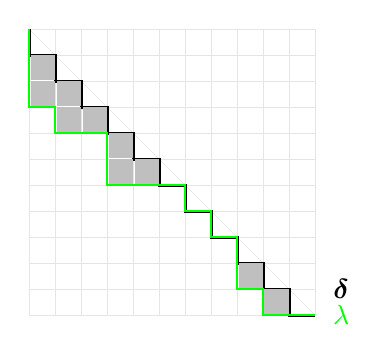
\begin{tikzpicture}[xscale = 0.33,yscale = 0.33]
      \draw[step=1cm,gray!20,very thin] (0,0) grid (11,11);
      \draw[step=1cm,gray!20,very thin] (0,11)--(11,0);
      \draw[very thick] (0,11)--(0,10)--(1,10)--(1,9)--(2,9)--(2,8)--(3,8)--(3,7)--(4,7)--(4,6)--(5,6)--(5,5)--(6,5)--(6,4)--(7,4)--(7,3)--(8,3)--(8,2)--(9,2)--(9,1)--(10,1)--(10,0)--(11,0);
      \draw[thick, green]
      (0,11)--(0,8)--(1,8)--(1,7)--(3,7)--(3,5)--(6,5)--(6,4)--(7,4)--(7,3)--(8,3)--(8,1)--(9,1)--(9,0)--(11,0);
      \node at (12,1) {$\bm{\delta}$};
      \node at (12,0) {\textcolor{green}{$\lambda$}};
      \foreach \point in
      {(0.05,10),(0.05,9),(1.05,9),(1.05,8),(2.05,8),(3.05,7),(3.05,6),(4.05,6),(8.05,2),(9.05,1)} {
        \fill[lightgray, visible on=<3->] \point -- +(0,-0.95) --
        +(0.95,-0.95) -- +(0.95,0) -- cycle;
      }
    \end{tikzpicture}
  \end{center}\pause
  \begin{itemize}
  \item \(\area(\lambda) = \) number of squares above \(\lambda\) but
    below the path \(\delta\) of alternating S-E steps. \pause
  \item E.g., above \(\area(\lambda) = 10\).\pause
  \item Catalan-number many Dyck paths for fixed \(k\). \pause (1,2,5,14,42,\ldots)
  \end{itemize}
\end{frame}
\begin{frame}
  \frametitle{dinv}
  \(\dinv(\lambda) = \)\# of balanced hooks in diagram below \(\lambda\).
   \begin{center}
    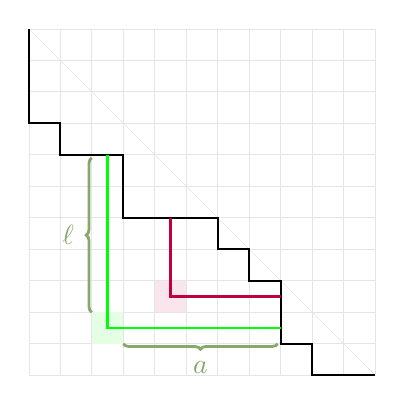
\begin{tikzpicture}[xscale = 0.4,yscale = 0.4]
	\draw[step=1cm,gray!20,very thin] (0,0) grid (11,11);
	\draw[step=1cm,gray!20,very thin] (0,11)--(11,0);
	\draw[thick] (0,11)--(0,8)--(1,8)--(1,7)--(3,7)--(3,5)--(6,5)--(6,4)--(7,4)--(7,3)--(8,3)--(8,1)--(9,1)--(9,0)--(11,0);
        \fill[purple!10] (4,3)--(5,3)--(5,2)--(4,2)--cycle;
        \draw[thick,purple] (4.5,5)--(4.5,2.5)--(8,2.5);
        \fill[green!10] (2,2)--(3,2)--(3,1)--(2,1)--cycle;
        \draw[thick,green] (2.5,7)--(2.5,1.5)--(8,1.5);

        \draw [decorate, asparagus, decoration={brace, mirror, amplitude=2pt}, line
        width=1pt, visible on=<2->] (3,1)--(7.9,1) node [midway, yshift=-0.3cm]{$a$};
        \draw [decorate, asparagus, decoration={brace, amplitude=2pt}, line
        width=1pt, visible on=<2->] (2,2)--(2,6.9) node [midway, xshift=-0.3cm]{$\ell$};
	% \node[left] at (0,10.5) {$1$};
	% \node[left] at (0,9.5) {$3$};
	% \node[left] at (0,8.5) {$4$};
	% \node[left] at (1,7.5) {$1$};
	% \node[left] at (3,6.5) {$3$};
	% \node[left] at (3,5.5) {$5$};
	% \node[left] at (6,4.5) {$2$};
	% \node[left] at (7,3.5) {$1$};
	% \node[left] at (8,2.5) {$1$};
	% \node[left] at (8,1.5) {$6$};
	% \node[left] at (9,0.5) {$4$};
	% \node[left,gray!60] at (11,-0.5) {$1$};
	% \node[left,gray!60] at (10,-0.5) {$2$};
	% \node[left,gray!60] at (9,-0.5) {$3$};
	% \node[left,gray!60] at (8,-0.5) {$4$};
	% \node[left,gray!60] at (7,-0.5) {$5$};
	% \node[left,gray!60] at (6,-0.5) {$6$};
	% \node[left,gray!60] at (5,-0.5) {$7$};
	% \node[left,gray!60] at (4,-0.5) {$8$};
	% \node[left,gray!60] at (3,-0.5) {$9$};
	% \node[left,gray!60] at (2,-0.5) {$10$};
	% \node[left,gray!60] at (1,-0.5) {$11$};
	% \node[left,gray!60] at (0,-0.5) {$j$};
	% \node[left] at (11,-1.5) {$0$};
	% \node[left] at (10,-1.5) {$1$};
	% \node[left] at (9,-1.5) {$1$};
	% \node[left] at (8,-1.5) {$0$};
	% \node[left] at (7,-1.5) {$0$};
	% \node[left] at (6,-1.5) {$0$};
	% \node[left] at (5,-1.5) {$1$};
	% \node[left] at (4,-1.5) {$2$};
	% \node[left] at (3,-1.5) {$1$};
	% \node[left] at (2,-1.5) {$2$};
	% \node[left] at (1,-1.5) {$2$};
	% \node[left] at (0,-1.5) {$c_j$};
	% \node[right,gray!60] at (11.2,11.5){$i$};
	% \node[right,gray!60] at (11.2,10.5){$1$};
	% \node[right,gray!60] at (11.2,9.5) {$2$};
	% \node[right,gray!60] at (11.2,8.5) {$3$};
	% \node[right,gray!60] at (11.2,7.5) {$4$};
	% \node[right,gray!60] at (11.2,6.5) {$5$};
	% \node[right,gray!60] at (11.2,5.5) {$6$};
	% \node[right,gray!60] at (11.2,4.5) {$7$};
	% \node[right,gray!60] at (11.2,3.5) {$8$};
	% \node[right,gray!60] at (11.2,2.5) {$9$};
	% \node[right,gray!60] at (11,1.5) {$10$};
	% \node[right,gray!60] at (11,0.5) {$11$};
	% \node at (14.3,11.5) {$r_i$};
	% \node at (14.2,10.5) {$0$};
	% \node at (14.2,9.5) {$1$};
	% \node at (14.2,8.5) {$2$};
	% \node at (14.2,7.5) {$2$};
	% \node at (14.2,6.5) {$1$};
	% \node at (14.2,5.5) {$2$};
	% \node at (14.2,4.5) {$0$};
	% \node at (14.2,3.5) {$0$};
	% \node at (14.2,2.5) {$0$};
	% \node at (14.2,1.5) {$1$};
	% \node at (14.2,0.5) {$1$};
\end{tikzpicture}
\end{center} \pause
Balanced hook is given by a cell below \(\lambda\) satisfying \[
  \frac{\ell}{a+1} < 1-\epsilon < \frac{\ell+1}{a}\,,\quad \epsilon
  \text{ small}.
\]
\end{frame}
\begin{frame}
  \frametitle{LLT Polynomials}
  Defined in general for a tuple of skew shapes \(\nu = (\nu^{(1)},\ldots,\nu^{(r)})\)\pause
  \begin{itemize}
  \item \(\Gcal_\nu(X;q)\) is a symmetric function\pause
  \item \(\Gcal_\nu(X;1) = s_{\nu^{(1)}} \cdots s_{\nu^{(r)}}\)\pause
  \item \(\Gcal_\nu\) were originally defined by Lascoux, Leclerc, and
    Thibon to explore connections to Fock space representations of \(U_q(\hat{\sl_r})\)\pause
  \item When \(\nu^{(i)}\) are partitions, the Schur-expansion
    coefficients are essentially parabolic Kazdhan-Luzstig polynomials.\pause
  \item \(\Gcal_\nu\) is Schur-positive for any tuple of skew shapes \(\nu\)
    [Grojnowski-Haiman, 2007].
  \end{itemize}
\end{frame}
\begin{frame}[fragile]
  \frametitle{LLT Polynomials}
  \(G_{\nu(\lambda)}(X;q)\) is an LLT polynomial for a tuple of rows,
  \(\nu(\lambda) = (\nu^{(1)},\ldots,\nu^{(r)})\).\pause \\
  \begin{center}
    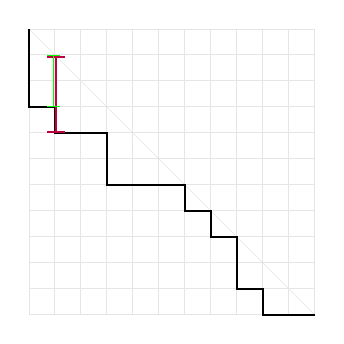
\begin{tikzpicture}[xscale = 0.33,yscale = 0.33]
      \draw[step=1cm,gray!20,very thin] (0,0) grid (11,11);
      \draw[step=1cm,gray!20,very thin] (0,11)--(11,0); \draw[thick]
      (0,11)--(0,8)--(1,8)--(1,7)--(3,7)--(3,5)--(6,5)--(6,4)--(7,4)--(7,3)--(8,3)--(8,1)--(9,1)--(9,0)--(11,0);
      \draw[|-|,thick,purple,visible on=<5->] (1.05,9.95)--(1.05,7);
      \draw[|-|,green,visible on=<4->] (0.95,10)--(0.95,8);
    \end{tikzpicture}\pause
    \raisebox{6em}{\(\to\)}
    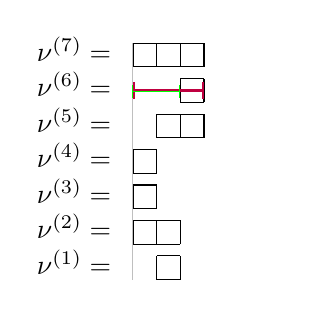
\begin{tikzpicture}[scale=.3]
       \newcommand{\drawRowp}[4]{ \def\r{#1};
        \def\a{#2}; \def\b{#3}; \def\labels{#4}; \draw
        [shift={(0,1.5*\r)}] (\b+2,1) grid (\a+2,0); \node at
        (-0.5,1.5*\r+0.75)
        {$\footnotesize \nu^{(\the\numexpr(\r+1)\relax)} = $};
        \setcounter{cp}{\a+1}; \foreach \nn in \labels { \node at
          (\thecp+1.5,1.5*\r+.5) {$\footnotesize \nn$};
          \addtocounter{cp}{1}; } };
      \draw[very thin, lightgray] (1.95,10)--(1.95,0);
      \drawRowp{6}{0}{3}{}
      \drawRowp{5}{2}{3}{} \drawRowp{4}{1}{3}{}
      \drawRowp{3}{0}{1}{}
      \drawRowp{2}{0}{1}{} \drawRowp{1}{0}{2}{} \drawRowp{0}{1}{2}{}
      % For spacing to center the tableau, not the = sign.
      \node at (8.5,8) {$\,$};
      \draw[|-|,thick,purple,visible on=<5->] (2,8)--(5,8);
      \draw[|-|,green,visible on=<4->] (1.95,7.95)--(4,7.95);
    \end{tikzpicture}
  \end{center}
\end{frame}
\begin{frame}[fragile]
  \frametitle{LLT Polynomials}
  \[
    \Gcal_\nu(X;q) = \sum_{T \in \SSYT(\nu)} q^{i(T)} x^T
  \]
  for \(T\) a weakly increasing filling of rows and \(i(T)\) the number of attacking inversions:\pause
  \vspace{-4.5em}
  \[
    T = 
     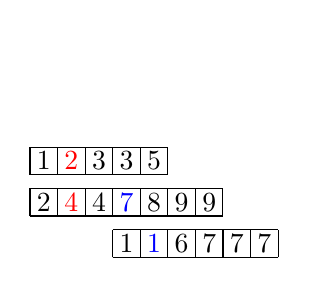
\begin{tikzpicture}[scale=.35]
      \newcommand{\drawRow}[4]{ \def\r{#1}; \def\a{#2}; \def\b{#3};
        \def\labels{#4}; \draw [shift={(0,1.5*\r)}] (\b+2,1) grid
        (\a+2,0); 
        \setcounter{c}{\a+1}; \foreach
        \nn in \labels {\node at (\thec+1.5,1.5*\r+.5) {
            $\footnotesize \nn$};
          \addtocounter{c}{1}; } };
      \drawRow{2}{0}{5}{1,{\textcolor{red}{2}},3,3,5} \drawRow{1}{0}{7}{2,\textcolor{red}{4},4,\textcolor{blue}{7},8,9,9} \drawRow{0}{3}{9}{1,\textcolor{blue}{1},6,7,7,7}
      % For spacing to center the tableau, not the = sign.
      \node at (8.5,8) {$\,$};
    \end{tikzpicture}\,\pause\to q^{i(T)}x^T = q^{18}x_1^3x_2^2x_3^2x_4^2x_5x_6x_7^4x_8x_9^2
  \]\pause
  \begin{itemize}
  \item \vspace{-2em}  
    \begin{align*} 
      \Gcal_{
        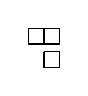
\begin{tikzpicture}[scale=0.2]
      \newcommand{\drawRow}[4]{ \def\r{#1}; \def\a{#2}; \def\b{#3};
        \def\labels{#4}; \draw [shift={(0,1.5*\r)}] (\b+2,1) grid
        (\a+2,0); 
        \setcounter{c}{\a+1}; \foreach
        \nn in \labels {\node at (\thec+1.5,1.5*\r+.5) {
            $\footnotesize \nn$};
          \addtocounter{c}{1}; } };
          \drawRow{1}{0}{2}{}
          \drawRow{0}{1}{2}{}
        \end{tikzpicture}
      }(x_1,x_2;q) =& x_1^3+x_1^2x_2+x_1x_2^2+x_2^3+qx_1^2x_2+qx_1x_2^2\\
                   &
        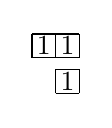
\begin{tikzpicture}[scale=0.3]
      \newcommand{\drawRow}[4]{ \def\r{#1}; \def\a{#2}; \def\b{#3};
        \def\labels{#4}; \draw [shift={(0,1.5*\r)}] (\b+2,1) grid
        (\a+2,0); 
        \setcounter{c}{\a+1}; \foreach
        \nn in \labels {\node at (\thec+1.5,1.5*\r+.5) {
            $\footnotesize \nn$};
          \addtocounter{c}{1}; } };
          \drawRow{1}{0}{2}{1,1}
          \drawRow{0}{1}{2}{1}
        \end{tikzpicture}
                     \phantom{+}
        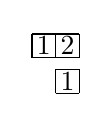
\begin{tikzpicture}[scale=0.3]
      \newcommand{\drawRow}[4]{ \def\r{#1}; \def\a{#2}; \def\b{#3};
        \def\labels{#4}; \draw [shift={(0,1.5*\r)}] (\b+2,1) grid
        (\a+2,0); 
        \setcounter{c}{\a+1}; \foreach
        \nn in \labels {\node at (\thec+1.5,1.5*\r+.5) {
            $\footnotesize \nn$};
          \addtocounter{c}{1}; } };
          \drawRow{1}{0}{2}{1,2}
          \drawRow{0}{1}{2}{1}
        \end{tikzpicture}
                     \phantom{+}
        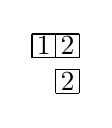
\begin{tikzpicture}[scale=0.3]
      \newcommand{\drawRow}[4]{ \def\r{#1}; \def\a{#2}; \def\b{#3};
        \def\labels{#4}; \draw [shift={(0,1.5*\r)}] (\b+2,1) grid
        (\a+2,0); 
        \setcounter{c}{\a+1}; \foreach
        \nn in \labels {\node at (\thec+1.5,1.5*\r+.5) {
            $\footnotesize \nn$};
          \addtocounter{c}{1}; } };
          \drawRow{1}{0}{2}{1,2}
          \drawRow{0}{1}{2}{2}
        \end{tikzpicture}
                     \phantom{+}
        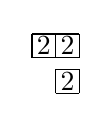
\begin{tikzpicture}[scale=0.3]
      \newcommand{\drawRow}[4]{ \def\r{#1}; \def\a{#2}; \def\b{#3};
        \def\labels{#4}; \draw [shift={(0,1.5*\r)}] (\b+2,1) grid
        (\a+2,0); 
        \setcounter{c}{\a+1}; \foreach
        \nn in \labels {\node at (\thec+1.5,1.5*\r+.5) {
            $\footnotesize \nn$};
          \addtocounter{c}{1}; } };
          \drawRow{1}{0}{2}{2,2}
          \drawRow{0}{1}{2}{2}
        \end{tikzpicture}
                     \phantom{+}
        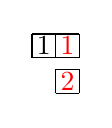
\begin{tikzpicture}[scale=0.3]
      \newcommand{\drawRow}[4]{ \def\r{#1}; \def\a{#2}; \def\b{#3};
        \def\labels{#4}; \draw [shift={(0,1.5*\r)}] (\b+2,1) grid
        (\a+2,0); 
        \setcounter{c}{\a+1}; \foreach
        \nn in \labels {\node at (\thec+1.5,1.5*\r+.5) {
            $\footnotesize \nn$};
          \addtocounter{c}{1}; } };
          \drawRow{1}{0}{2}{1,\textcolor{red}{1}}
          \drawRow{0}{1}{2}{\textcolor{red}{2}}
        \end{tikzpicture}
                     \phantom{+}
        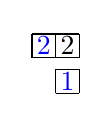
\begin{tikzpicture}[scale=0.3]
      \newcommand{\drawRow}[4]{ \def\r{#1}; \def\a{#2}; \def\b{#3};
        \def\labels{#4}; \draw [shift={(0,1.5*\r)}] (\b+2,1) grid
        (\a+2,0); 
        \setcounter{c}{\a+1}; \foreach
        \nn in \labels {\node at (\thec+1.5,1.5*\r+.5) {
            $\footnotesize \nn$};
          \addtocounter{c}{1}; } };
          \drawRow{1}{0}{2}{\textcolor{blue}{2},2}
          \drawRow{0}{1}{2}{\textcolor{blue}{1}}
        \end{tikzpicture}\\
       = & s_3+qs_{2,1}
    \end{align*}
    \vspace{-0.5em}
  \end{itemize}
\end{frame}
\begin{frame}
  \frametitle{Example \(\nabla e_3\)}
  \vspace{-2em}
  \begin{eqnarray*}
    \lambda
    & q^{\dinv(\lambda)}t^{\area(\lambda)}
    & q^{\dinv(\lambda)}t^{\area(\lambda)}\Gcal_{\nu(\lambda)}(X;q^{-1})\\
      \onslide<2->{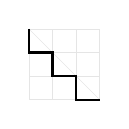
\begin{tikzpicture}[xscale = 0.3,yscale = 0.3]
      \draw[step=1cm,gray!20,very thin] (0,0) grid (3,3);
      \draw[step=1cm,gray!20,very thin] (0,3)--(3,0); \draw[thick]
      (0,3)--(0,2)--(1,2)--(1,1)--(2,1)--(2,0)--(3,0);
    \end{tikzpicture}}
    & \onslide<3->{q^3}
    & \onslide<4->{s_3+qs_{2,1}+q^2s_{2,1}+q^3s_{1,1,1}}\\
    \onslide<2->
    {
    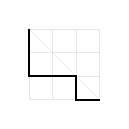
\begin{tikzpicture}[xscale = 0.3,yscale = 0.3]
      \draw[step=1cm,gray!20,very thin] (0,0) grid (3,3);
      \draw[step=1cm,gray!20,very thin] (0,3)--(3,0); \draw[thick]
      (0,3)--(0,1)--(2,1)--(2,0)--(3,0);
    \end{tikzpicture}
    }
    & \onslide<3->{q^2t}
    & \onslide<4->{\phantom{ts_{2,1}+}qts_{2,1}+q^2ts_{1,1,1}}  \\
    \onslide<2->
    {
    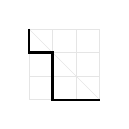
\begin{tikzpicture}[xscale = 0.3,yscale = 0.3]
      \draw[step=1cm,gray!20,very thin] (0,0) grid (3,3);
      \draw[step=1cm,gray!20,very thin] (0,3)--(3,0); \draw[thick]
      (0,3)--(0,2)--(1,2)--(1,0)--(3,0);
    \end{tikzpicture}
    }
    & \onslide<3->{qt}
    & \onslide<4->{ts_{2,1}+qts_{1,1,1}}\\
    \onslide<2->
    {
    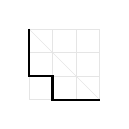
\begin{tikzpicture}[xscale = 0.3,yscale = 0.3]
      \draw[step=1cm,gray!20,very thin] (0,0) grid (3,3);
      \draw[step=1cm,gray!20,very thin] (0,3)--(3,0); \draw[thick]
      (0,3)--(0,1)--(1,1)--(1,0)--(3,0);
    \end{tikzpicture}
    }
    &\onslide<3->{qt^2}
    &\onslide<4->{ t^2 s_{2,1}+qt^2s_{1,1,1}}\\
    \onslide<2->
    {
    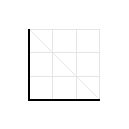
\begin{tikzpicture}[xscale = 0.3,yscale = 0.3]
      \draw[step=1cm,gray!20,very thin] (0,0) grid (3,3);
      \draw[step=1cm,gray!20,very thin] (0,3)--(3,0); \draw[thick]
      (0,3)--(0,0)--(3,0);
    \end{tikzpicture}
    }
    &\onslide<3->{t^3}
    & \onslide<4->{t^3s_{1,1,1}}
  \end{eqnarray*}
  \vspace{-0.75em}
  \begin{itemize}
  \item<5-> Entire quantity is \(q,t\)-symmetric
  \item<6-> Coefficient of \(s_{1,1,1}\) in sum is a ``\((q,t)\)-Catalan
    number'' \((q^3+q^2t+qt+qt^2+t^3)\)\,.
  \end{itemize}
\end{frame}
\begin{frame}{Generalizing Shuffle Theorem}
  When a problem is too difficult, try generalizing! \pause
  \begin{eqnarray*}
    \text{Algebraic Expression} & \text{Combinatorial Expression}\\
    \nabla e_k(X) & = \sum q,t\text{-weighted Dyck paths}\\
  \end{eqnarray*}\pause
  \vspace{-5ex}
   \begin{block}{Rational Shuffle Conjecture (F. Bergeron, Garsia,
      Sergel Leven, Xin, 2016) (Proved by Mellit, 2016)}
    For \(m,n\) coprime, the operator \(e_k[-MX^{m,n}]\) acting on
    \(\sym\) satisfies \[
      e_k[-M X^{m,n}] \cdot 1 = \sum q,t\text{-weighted
      }(km,kn)\text{-Dyck paths}
    \]
    \end{block}\pause
    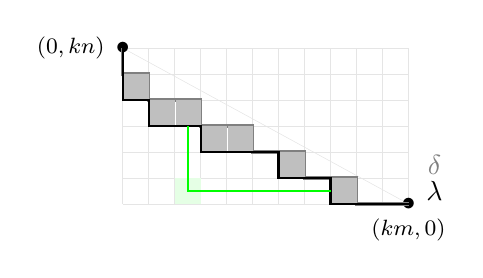
\begin{tikzpicture}[xscale = 0.33,yscale = 0.33]
      \draw[step=1cm,gray!20,very thin] (0,0) grid (11,6);
      \draw[step=1cm,gray!20,very thin] (0,6)--(11,0);
      \node at (0,6) {$\bullet$};
      \node at (11,0) {$\bullet$};
      \draw[very thick, gray] (0,6)--(0,5)--(1,5)--(1,4)--(3,4)--(3,3)--(5,3)--(5,2)--(7,2)--(7,1)--(9,1)--(9,0)--(11,0);
      \draw[thick]
      (0,6)--(0,4)--(1,4)--(1,3)--(3,3)--(3,2)--(6,2)--(6,1)--(8,1)--(8,0)--(11,0);
      \node at (12,1.5) {\textcolor{gray}{$\delta$}};
      \node at (12,0.5) {$\lambda$};
      \node at (-2,6) {\footnotesize $(0,kn)$};
      \node at (11,-1) {\footnotesize $(km,0)$};
      \foreach \point in
      {(0.05,5),(1.05,4),(2.05,4),(3.05,3),(4.05,3),(6.05,2),(8.05,1)}
      {
        \fill[lightgray, visible on=<2->] \point -- +(0,-0.95) --
        +(0.95,-0.95) -- +(0.95,0) -- cycle;
      }
      \fill[green!10, visible on=<3->] (2,1)--(3,1)--(3,0)--(2,0)--cycle;
      \draw[thick,green, visible on=<3->] (2.5,3)--(2.5,0.5)--(8,0.5);
    \end{tikzpicture}
\end{frame}
\begin{frame}{Welcome to the Zoo}
  \begin{itemize}
  \item The operators \(e_k[-MX^{m,n}]\) arise from an action of
    \emph{Schiffmann algebra} \(\Ecal\) on \(\Lambda\). \pause
  \item \(\Ecal\) contains subalgebra
    \(\Lambda(X^{m,n}) \isom \Lambda\) for each coprime pair
    \((m,n) \in \Z^2\).\pause
  \item In general, \(\Ecal\)-action can be a pain to compute in a
    nice way, but
    sometimes it is nice!
  \end{itemize}
  \begin{equation*}
  % \begin{tikzcd}
  %   \Ecal \ar[r,"\text{acts on}"] & \Lambda
  % \end{tikzcd}
\end{equation*}
\end{frame}
\begin{frame}{Welcome to the Zoo: Catalanimals}
  Fix \(l \in \Z_{>0}\). Let \(R_+ = \{(i,j) \st 1 \leq i < j \leq l\}\) .\pause
  \begin{definition}
    For subsets \(R_q, R_t, R_{qt} \subset R_+\) and \(\gamma \in
    \Z^l\), a \emph{Catalanimal} \(H = H(R_q,R_t,R_{qt},\gamma)(z_1,\ldots,z_l;q,t)\) is a
    symmetric rational function\pause
    \[
 \sum_{w \in S_l} w \left(
        \frac{z_1^{\gamma_1} \cdots z_l^{\gamma_l} \prod_{(i,j) \in
            R_{qt}} (1 - qt z_i/z_j)}{\prod_{(i,j) \in R_+}
          (1-z_j/z_i) \prod_{(i,j) \in R_q} (1-q z_i/z_j) \prod_{(i,j)
          \in R_t} (1-t z_i/z_j)} \right)
    \]
  \end{definition}
\pause
  \begin{itemize}
  \item Can also be thought of as an infinite series of virtual \(GL_l\)-characters.\pause
  \item We can take ``polynomial part'' (restrict to only polynomial
    \(GL_l\)-characters) to get a symmetric function.
  \end{itemize}
\end{frame}
\begin{frame}{Welcome to the Zoo: Catalanimals}
  \begin{itemize}
  \item Visual representations of Catalanimals are less scary.\pause
  \item Assume \(R_{qt} \subset R_t \subset R_q \subset R_+\):\pause
  \end{itemize}
\[
\begin{array}{@{\hspace{0.2mm}}c@{\quad\quad}cr}
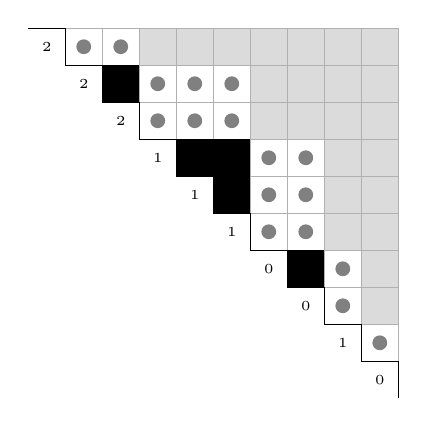
\begin{tikzpicture}[scale = .47]
\begin{scope}
\draw[draw = none, fill = black!14] (4,-1) rectangle (5,-2);
 \draw[draw = none, fill = black!14] (5,-1) rectangle (6,-2);
 \draw[draw = none, fill = black!14] (6,-1) rectangle (7,-2);
 \draw[draw = none, fill = black!14] (7,-1) rectangle (8,-2);
 \draw[draw = none, fill = black!14] (7,-2) rectangle (8,-3);
 \draw[draw = none, fill = black!14] (7,-3) rectangle (8,-4);
 \draw[draw = none, fill = black!14] (8,-1) rectangle (9,-2);
 \draw[draw = none, fill = black!14] (8,-2) rectangle (9,-3);
 \draw[draw = none, fill = black!14] (8,-3) rectangle (9,-4);
 \draw[draw = none, fill = black!14] (9,-1) rectangle (10,-2);
 \draw[draw = none, fill = black!14] (9,-2) rectangle (10,-3);
 \draw[draw = none, fill = black!14] (9,-3) rectangle (10,-4);
 \draw[draw = none, fill = black!14] (9,-4) rectangle (10,-5);
 \draw[draw = none, fill = black!14] (9,-5) rectangle (10,-6);
 \draw[draw = none, fill = black!14] (9,-6) rectangle (10,-7);
 \draw[draw = none, fill = black!14] (10,-1) rectangle (11,-2);
 \draw[draw = none, fill = black!14] (10,-2) rectangle (11,-3);
 \draw[draw = none, fill = black!14] (10,-3) rectangle (11,-4);
 \draw[draw = none, fill = black!14] (10,-4) rectangle (11,-5);
 \draw[draw = none, fill = black!14] (10,-5) rectangle (11,-6);
 \draw[draw = none, fill = black!14] (10,-6) rectangle (11,-7);
 \draw[draw = none, fill = black!14] (10,-7) rectangle (11,-8);
 \draw[draw = none, fill = black!14] (10,-8) rectangle (11,-9);
 \draw[draw = none, fill = gray!100] (2+0.5, -1-0.5) circle (.2);
\draw[draw = none, fill = gray!100] (3+0.5, -1-0.5) circle (.2);
\draw[draw = none, fill = gray!100] (4+0.5, -2-0.5) circle (.2);
\draw[draw = none, fill = gray!100] (5+0.5, -2-0.5) circle (.2);
\draw[draw = none, fill = gray!100] (6+0.5, -2-0.5) circle (.2);
\draw[draw = none, fill = gray!100] (4+0.5, -3-0.5) circle (.2);
\draw[draw = none, fill = gray!100] (5+0.5, -3-0.5) circle (.2);
\draw[draw = none, fill = gray!100] (6+0.5, -3-0.5) circle (.2);
\draw[draw = none, fill = gray!100] (7+0.5, -4-0.5) circle (.2);
\draw[draw = none, fill = gray!100] (8+0.5, -4-0.5) circle (.2);
\draw[draw = none, fill = gray!100] (7+0.5, -5-0.5) circle (.2);
\draw[draw = none, fill = gray!100] (8+0.5, -5-0.5) circle (.2);
\draw[draw = none, fill = gray!100] (7+0.5, -6-0.5) circle (.2);
\draw[draw = none, fill = gray!100] (8+0.5, -6-0.5) circle (.2);
\draw[draw = none, fill = gray!100] (9+0.5, -7-0.5) circle (.2);
\draw[draw = none, fill = gray!100] (9+0.5, -8-0.5) circle (.2);
\draw[draw = none, fill = gray!100] (10+0.5, -9-0.5) circle (.2);
\draw[thin, black!31] (1,-1) -- (11,-1);
\draw[thin, black!31] (2,-1) -- (2,-1);
\draw[thin, black!31] (2,-2) -- (11,-2);
\draw[thin, black!31] (3,-2) -- (3,-1);
\draw[thin, black!31] (3,-3) -- (11,-3);
\draw[thin, black!31] (4,-3) -- (4,-1);
\draw[thin, black!31] (4,-4) -- (11,-4);
\draw[thin, black!31] (5,-4) -- (5,-1);
\draw[thin, black!31] (5,-5) -- (11,-5);
\draw[thin, black!31] (6,-5) -- (6,-1);
\draw[thin, black!31] (6,-6) -- (11,-6);
\draw[thin, black!31] (7,-6) -- (7,-1);
\draw[thin, black!31] (7,-7) -- (11,-7);
\draw[thin, black!31] (8,-7) -- (8,-1);
\draw[thin, black!31] (8,-8) -- (11,-8);
\draw[thin, black!31] (9,-8) -- (9,-1);
\draw[thin, black!31] (9,-9) -- (11,-9);
\draw[thin, black!31] (10,-9) -- (10,-1);
\draw[thin, black!31] (10,-10) -- (11,-10);
\draw[thin, black!31] (11,-10) -- (11,-1);
\draw[draw = none, fill = black!100] (3,-2) rectangle (4,-3);
 \draw[draw = none, fill = black!100] (5,-4) rectangle (6,-5);
 \draw[draw = none, fill = black!100] (6,-4) rectangle (7,-5);
 \draw[draw = none, fill = black!100] (6,-5) rectangle (7,-6);
 \draw[draw = none, fill = black!100] (8,-7) rectangle (9,-8);
 \draw[thin] (1,-1) -- (2,-1);
\draw[thin] (2,-1) -- (2,-2);
\draw[thin] (2,-2) -- (3,-2);
\draw[thin] (3,-2) -- (3,-3);
\draw[thin] (3,-3) -- (4,-3);
\draw[thin] (4,-3) -- (4,-4);
\draw[thin] (4,-4) -- (5,-4);
\draw[thin] (5,-4) -- (5,-5);
\draw[thin] (5,-5) -- (6,-5);
\draw[thin] (6,-5) -- (6,-6);
\draw[thin] (6,-6) -- (7,-6);
\draw[thin] (7,-6) -- (7,-7);
\draw[thin] (7,-7) -- (8,-7);
\draw[thin] (8,-7) -- (8,-8);
\draw[thin] (8,-8) -- (9,-8);
\draw[thin] (9,-8) -- (9,-9);
\draw[thin] (9,-9) -- (10,-9);
\draw[thin] (10,-9) -- (10,-10);
\draw[thin] (10,-10) -- (11,-10);
\draw[thin] (11,-10) -- (11,-11);
\node at (3/2,-3/2) {\tiny $2 $};
\node at (5/2,-5/2) {\tiny $2 $};
\node at (7/2,-7/2) {\tiny $2 $};
\node at (9/2,-9/2) {\tiny $1 $};
\node at (11/2,-11/2) {\tiny $1 $};
\node at (13/2,-13/2) {\tiny $1 $};
\node at (15/2,-15/2) {\tiny $0 $};
\node at (17/2,-17/2) {\tiny $0 $};
\node (vv) at (19/2,-19/2) {\tiny $1 $};
\node at (21/2,-21/2) {\tiny $0 $};
\end{scope}
\end{tikzpicture}
&  
\raisebox{9mm}{
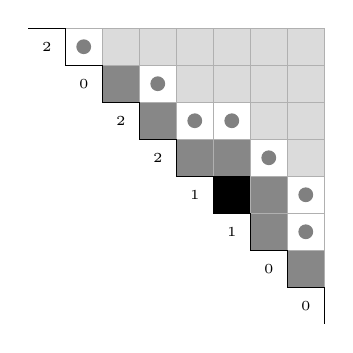
\begin{tikzpicture}[scale=.47]
\begin{scope}
\draw[draw = none, fill = black!14] (3,-1) rectangle (4,-2);
 \draw[draw = none, fill = black!14] (4,-1) rectangle (5,-2);
 \draw[draw = none, fill = black!14] (5,-1) rectangle (6,-2);
 \draw[draw = none, fill = black!14] (5,-2) rectangle (6,-3);
 \draw[draw = none, fill = black!14] (6,-1) rectangle (7,-2);
 \draw[draw = none, fill = black!14] (6,-2) rectangle (7,-3);
 \draw[draw = none, fill = black!14] (7,-1) rectangle (8,-2);
 \draw[draw = none, fill = black!14] (7,-2) rectangle (8,-3);
 \draw[draw = none, fill = black!14] (7,-3) rectangle (8,-4);
 \draw[draw = none, fill = black!14] (8,-1) rectangle (9,-2);
 \draw[draw = none, fill = black!14] (8,-2) rectangle (9,-3);
 \draw[draw = none, fill = black!14] (8,-3) rectangle (9,-4);
 \draw[draw = none, fill = black!14] (8,-4) rectangle (9,-5);
 \draw[draw = none, fill = gray!100] (2+0.5, -1-0.5) circle (.2);
\draw[draw = none, fill = gray!100] (4+0.5, -2-0.5) circle (.2);
\draw[draw = none, fill = gray!100] (5+0.5, -3-0.5) circle (.2);
\draw[draw = none, fill = gray!100] (6+0.5, -3-0.5) circle (.2);
\draw[draw = none, fill = gray!100] (7+0.5, -4-0.5) circle (.2);
\draw[draw = none, fill = gray!100] (8+0.5, -5-0.5) circle (.2);
\draw[draw = none, fill = gray!100] (8+0.5, -6-0.5) circle (.2);
\draw[draw = none, fill = \mymidgray] (3,-2) rectangle (4,-3);
 \draw[draw = none, fill = \mymidgray] (4,-3) rectangle (5,-4);
 \draw[draw = none, fill = \mymidgray] (5,-4) rectangle (6,-5);
 \draw[draw = none, fill = \mymidgray] (6,-4) rectangle (7,-5);
 \draw[draw = none, fill = \mymidgray] (7,-5) rectangle (8,-6);
 \draw[draw = none, fill = \mymidgray] (7,-6) rectangle (8,-7);
 \draw[draw = none, fill = \mymidgray] (8,-7) rectangle (9,-8);
 \draw[thin, black!31] (1,-1) -- (9,-1);
\draw[thin, black!31] (2,-1) -- (2,-1);
\draw[thin, black!31] (2,-2) -- (9,-2);
\draw[thin, black!31] (3,-2) -- (3,-1);
\draw[thin, black!31] (3,-3) -- (9,-3);
\draw[thin, black!31] (4,-3) -- (4,-1);
\draw[thin, black!31] (4,-4) -- (9,-4);
\draw[thin, black!31] (5,-4) -- (5,-1);
\draw[thin, black!31] (5,-5) -- (9,-5);
\draw[thin, black!31] (6,-5) -- (6,-1);
\draw[thin, black!31] (6,-6) -- (9,-6);
\draw[thin, black!31] (7,-6) -- (7,-1);
\draw[thin, black!31] (7,-7) -- (9,-7);
\draw[thin, black!31] (8,-7) -- (8,-1);
\draw[thin, black!31] (8,-8) -- (9,-8);
\draw[thin, black!31] (9,-8) -- (9,-1);
\draw[draw = none, fill = black!100] (6,-5) rectangle (7,-6);
 \draw[thin] (1,-1) -- (2,-1);
\draw[thin] (2,-1) -- (2,-2);
\draw[thin] (2,-2) -- (3,-2);
\draw[thin] (3,-2) -- (3,-3);
\draw[thin] (3,-3) -- (4,-3);
\draw[thin] (4,-3) -- (4,-4);
\draw[thin] (4,-4) -- (5,-4);
\draw[thin] (5,-4) -- (5,-5);
\draw[thin] (5,-5) -- (6,-5);
\draw[thin] (6,-5) -- (6,-6);
\draw[thin] (6,-6) -- (7,-6);
\draw[thin] (7,-6) -- (7,-7);
\draw[thin] (7,-7) -- (8,-7);
\draw[thin] (8,-7) -- (8,-8);
\draw[thin] (8,-8) -- (9,-8);
\draw[thin] (9,-8) -- (9,-9);
\node at (3/2,-3/2) {\tiny $2 $};
\node at (5/2,-5/2) {\tiny $0 $};
\node at (7/2,-7/2) {\tiny $2 $};
\node at (9/2,-9/2) {\tiny $2 $};
\node at (11/2,-11/2) {\tiny $1 $};
\node at (13/2,-13/2) {\tiny $1 $};
\node at (15/2,-15/2) {\tiny $0 $};
\node (vv) at (17/2,-17/2) {\tiny $0 $};
\end{scope}
\end{tikzpicture} }
&
\ \ \
\raisebox{16mm}{
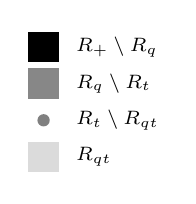
\begin{tikzpicture}[scale = .39]
\begin{scope}
\draw[draw = none, fill = black!100] (2,-1) rectangle (3,-2);
\node[anchor = west] at (3,-1.5) {\scriptsize  \  $R_+ \setminus R_q$};
\end{scope}
\begin{scope}[yshift = -34*1]
\draw[draw = none, fill = \mymidgray] (2,-1) rectangle (3,-2);
\node[anchor = west] at (3,-1.5) {\scriptsize  \  $R_q \setminus R_t$};
\end{scope}
\begin{scope}[yshift = -34*2]
\draw[thin, black!0] (2,-1) -- (3,-1);
\draw[thin, black!0] (2,-1) -- (2,-2);
\draw[thin, black!0] (2,-2) -- (3,-2);
\draw[thin, black!0] (3,-2) -- (3,-1);
\draw[draw = none, fill = gray!100] (2+0.5, -1-0.5) circle (.2);
\node[anchor = west] at (3,-1.5) {\scriptsize  \  $R_t \setminus R_{qt}$};
\end{scope}
\begin{scope}[yshift = -34*3]
\draw[draw = none, fill = black!14] (2,-1) rectangle (3,-2);
\node[anchor = west] at (3,-1.5) {\scriptsize \  $R_{qt}$};
\end{scope}
\end{tikzpicture}}
\end{array}
\]
\end{frame}
\begin{frame}{Tame and cuddly Catalanimals}
  \begin{itemize}
  \item Sometimes, there exists \(\xi \in \Ecal\) such that \(\xi
    \cdot 1 = \omega \pol_X H\). \pause(!!!)\pause
  \item When \(R_{qt} \subset [R_q, R_t]\), then this
    happens. (Associated \(H\)
    is \emph{tame}.)\pause
  \item When, \(H\) is \emph{\((m,n)\)-cuddly} (a set of inequalities
    on root sets and weight), there
    exists an \(f \in \Lambda\) such that \(f[-MX^{m,n}] \cdot 1 =
    \omega \pol_X H\) (up to \(q,t\)-monomial and sign).\pause
  \item In this case, we set \(\operatorname{cub}(H) = f\).\pause
  \item The cuddly conditions allow a nice coproduct formula for
    \(f[X+Y]\) in terms of cubs of ``restrictions'' of \(H\).
  \end{itemize}
\end{frame}
\begin{frame}{Cuddly Catalanimals with cub \(e_k\)}
  \begin{itemize}
  \item \(H(R_+,R_+,[R_+,R_+],(1^k))\) is \((1,1)\)-cuddly with cub \(e_k\).\pause
  \item More generally, if \(\delta\) is the sequence of south step
    runs of highest path under the line through \((0,kn)\) to
    \((km,0)\), then \(e_k[-MX^{m,n}] \cdot 1 = H(R_+,R_+,[R_+,R_+],\delta)\).\pause
  \end{itemize}
  \[
  \begin{array}{c@{\quad\quad}cr}
  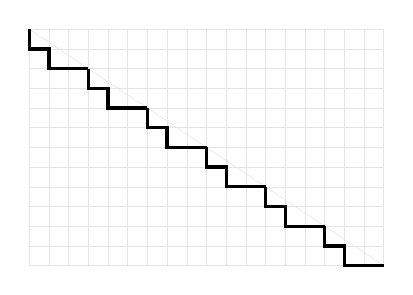
\begin{tikzpicture}[scale=0.25]
      \draw[step=1cm,gray!20,very thin] (0,0) grid (18,12);
      \draw[step=1cm,gray!20,very thin] (0,12)--(18,0);
      \foreach \off in {0,1,2,3,4,5} {
      \draw[very thick] (0+3*\off,12-2*\off)--(0+3*\off,11-2*\off)--(1+3*\off,11-2*\off)--(1+3*\off,10-2*\off)--(3+3*\off,10-2*\off);
      }
    \end{tikzpicture}
    &
      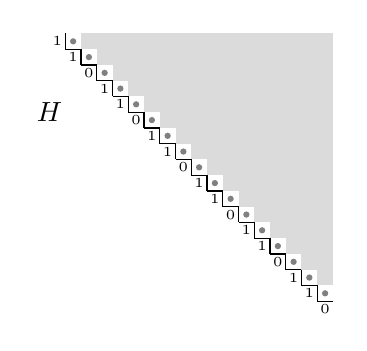
\begin{tikzpicture}[scale=0.2]
        \foreach \j in {1,...,17} {
          \draw[draw = none, fill = gray!100] (\j+0.5, -\j-0.5) circle (.2);
        }
        \foreach \j in {1,...,16} {
          \pgfmathsetmacro{\z}{\j+1}
          \foreach \i in {\z,...,17} {
            \draw[draw = none, fill = black!14] (\i,-\j) rectangle (\i+1,-\j-1);
          }
        }
        \draw[thin] (1,-1) -- (1,-2);
        \foreach \j in {2,...,17} {
          \draw[thin] (\j-1,-\j) -- (\j,-\j);
          \draw[thin] (\j,-\j) -- (\j,-\j-1);
        }
        \draw[thin] (17,-18) -- (18,-18);
        \foreach \j in {0,...,5} {
          \node at (3*\j+0.5,-3*\j-1.5) {\tiny \(1\)};
          \node at (3*\j+1.5,-3*\j-2.5) {\tiny \(1\)};
          \node at (3*\j+2.5,-3*\j-3.5) {\tiny \(0\)};
        }
        \node at (0,-6) {\(H\)};
      \end{tikzpicture}
      
    &\raisebox{16mm}{
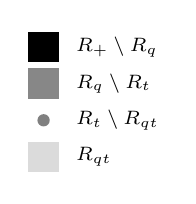
\begin{tikzpicture}[scale = .39]
\begin{scope}
\draw[draw = none, fill = black!100] (2,-1) rectangle (3,-2);
\node[anchor = west] at (3,-1.5) {\scriptsize  \  $R_+ \setminus R_q$};
\end{scope}
\begin{scope}[yshift = -34*1]
\draw[draw = none, fill = \mymidgray] (2,-1) rectangle (3,-2);
\node[anchor = west] at (3,-1.5) {\scriptsize  \  $R_q \setminus R_t$};
\end{scope}
\begin{scope}[yshift = -34*2]
\draw[thin, black!0] (2,-1) -- (3,-1);
\draw[thin, black!0] (2,-1) -- (2,-2);
\draw[thin, black!0] (2,-2) -- (3,-2);
\draw[thin, black!0] (3,-2) -- (3,-1);
\draw[draw = none, fill = gray!100] (2+0.5, -1-0.5) circle (.2);
\node[anchor = west] at (3,-1.5) {\scriptsize  \  $R_t \setminus R_{qt}$};
\end{scope}
\begin{scope}[yshift = -34*3]
\draw[draw = none, fill = black!14] (2,-1) rectangle (3,-2);
\node[anchor = west] at (3,-1.5) {\scriptsize \  $R_{qt}$};
\end{scope}
\end{tikzpicture}}
  \end{array}
  \]
  \(\delta = (1,1,0,1,1,0,1,1,0,1,1,0,1,1,0,1,1,0)\) and
  \(e_6[-MX^{3,2}] \cdot 1 = \omega \pol_X H\)
\end{frame}
\begin{frame}{\(1,1\)-Cuddly Catalanimals with cub \(s_\mu\)}
  \begin{itemize}
  \item Can construct root sets and weight from the content diagonals of \(\mu\).\pause
  \item \(\mu = \ydiagram{4,3,3} \to \ytableaushort{+..-,+.-,+.-}
    \to \ytableaushort{1010,210,221}\).\pause 
  \end{itemize}
  \[\begin{array}{cr}
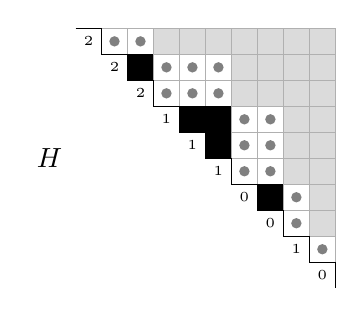
\begin{tikzpicture}[scale = .33]
\begin{scope}
\draw[draw = none, fill = black!14] (4,-1) rectangle (5,-2);
 \draw[draw = none, fill = black!14] (5,-1) rectangle (6,-2);
 \draw[draw = none, fill = black!14] (6,-1) rectangle (7,-2);
 \draw[draw = none, fill = black!14] (7,-1) rectangle (8,-2);
 \draw[draw = none, fill = black!14] (7,-2) rectangle (8,-3);
 \draw[draw = none, fill = black!14] (7,-3) rectangle (8,-4);
 \draw[draw = none, fill = black!14] (8,-1) rectangle (9,-2);
 \draw[draw = none, fill = black!14] (8,-2) rectangle (9,-3);
 \draw[draw = none, fill = black!14] (8,-3) rectangle (9,-4);
 \draw[draw = none, fill = black!14] (9,-1) rectangle (10,-2);
 \draw[draw = none, fill = black!14] (9,-2) rectangle (10,-3);
 \draw[draw = none, fill = black!14] (9,-3) rectangle (10,-4);
 \draw[draw = none, fill = black!14] (9,-4) rectangle (10,-5);
 \draw[draw = none, fill = black!14] (9,-5) rectangle (10,-6);
 \draw[draw = none, fill = black!14] (9,-6) rectangle (10,-7);
 \draw[draw = none, fill = black!14] (10,-1) rectangle (11,-2);
 \draw[draw = none, fill = black!14] (10,-2) rectangle (11,-3);
 \draw[draw = none, fill = black!14] (10,-3) rectangle (11,-4);
 \draw[draw = none, fill = black!14] (10,-4) rectangle (11,-5);
 \draw[draw = none, fill = black!14] (10,-5) rectangle (11,-6);
 \draw[draw = none, fill = black!14] (10,-6) rectangle (11,-7);
 \draw[draw = none, fill = black!14] (10,-7) rectangle (11,-8);
 \draw[draw = none, fill = black!14] (10,-8) rectangle (11,-9);
 \draw[draw = none, fill = gray!100] (2+0.5, -1-0.5) circle (.2);
\draw[draw = none, fill = gray!100] (3+0.5, -1-0.5) circle (.2);
\draw[draw = none, fill = gray!100] (4+0.5, -2-0.5) circle (.2);
\draw[draw = none, fill = gray!100] (5+0.5, -2-0.5) circle (.2);
\draw[draw = none, fill = gray!100] (6+0.5, -2-0.5) circle (.2);
\draw[draw = none, fill = gray!100] (4+0.5, -3-0.5) circle (.2);
\draw[draw = none, fill = gray!100] (5+0.5, -3-0.5) circle (.2);
\draw[draw = none, fill = gray!100] (6+0.5, -3-0.5) circle (.2);
\draw[draw = none, fill = gray!100] (7+0.5, -4-0.5) circle (.2);
\draw[draw = none, fill = gray!100] (8+0.5, -4-0.5) circle (.2);
\draw[draw = none, fill = gray!100] (7+0.5, -5-0.5) circle (.2);
\draw[draw = none, fill = gray!100] (8+0.5, -5-0.5) circle (.2);
\draw[draw = none, fill = gray!100] (7+0.5, -6-0.5) circle (.2);
\draw[draw = none, fill = gray!100] (8+0.5, -6-0.5) circle (.2);
\draw[draw = none, fill = gray!100] (9+0.5, -7-0.5) circle (.2);
\draw[draw = none, fill = gray!100] (9+0.5, -8-0.5) circle (.2);
\draw[draw = none, fill = gray!100] (10+0.5, -9-0.5) circle (.2);
\draw[thin, black!31] (1,-1) -- (11,-1);
\draw[thin, black!31] (2,-1) -- (2,-1);
\draw[thin, black!31] (2,-2) -- (11,-2);
\draw[thin, black!31] (3,-2) -- (3,-1);
\draw[thin, black!31] (3,-3) -- (11,-3);
\draw[thin, black!31] (4,-3) -- (4,-1);
\draw[thin, black!31] (4,-4) -- (11,-4);
\draw[thin, black!31] (5,-4) -- (5,-1);
\draw[thin, black!31] (5,-5) -- (11,-5);
\draw[thin, black!31] (6,-5) -- (6,-1);
\draw[thin, black!31] (6,-6) -- (11,-6);
\draw[thin, black!31] (7,-6) -- (7,-1);
\draw[thin, black!31] (7,-7) -- (11,-7);
\draw[thin, black!31] (8,-7) -- (8,-1);
\draw[thin, black!31] (8,-8) -- (11,-8);
\draw[thin, black!31] (9,-8) -- (9,-1);
\draw[thin, black!31] (9,-9) -- (11,-9);
\draw[thin, black!31] (10,-9) -- (10,-1);
\draw[thin, black!31] (10,-10) -- (11,-10);
\draw[thin, black!31] (11,-10) -- (11,-1);
\draw[draw = none, fill = black!100] (3,-2) rectangle (4,-3);
 \draw[draw = none, fill = black!100] (5,-4) rectangle (6,-5);
 \draw[draw = none, fill = black!100] (6,-4) rectangle (7,-5);
 \draw[draw = none, fill = black!100] (6,-5) rectangle (7,-6);
 \draw[draw = none, fill = black!100] (8,-7) rectangle (9,-8);
 \draw[thin] (1,-1) -- (2,-1);
\draw[thin] (2,-1) -- (2,-2);
\draw[thin] (2,-2) -- (3,-2);
\draw[thin] (3,-2) -- (3,-3);
\draw[thin] (3,-3) -- (4,-3);
\draw[thin] (4,-3) -- (4,-4);
\draw[thin] (4,-4) -- (5,-4);
\draw[thin] (5,-4) -- (5,-5);
\draw[thin] (5,-5) -- (6,-5);
\draw[thin] (6,-5) -- (6,-6);
\draw[thin] (6,-6) -- (7,-6);
\draw[thin] (7,-6) -- (7,-7);
\draw[thin] (7,-7) -- (8,-7);
\draw[thin] (8,-7) -- (8,-8);
\draw[thin] (8,-8) -- (9,-8);
\draw[thin] (9,-8) -- (9,-9);
\draw[thin] (9,-9) -- (10,-9);
\draw[thin] (10,-9) -- (10,-10);
\draw[thin] (10,-10) -- (11,-10);
\draw[thin] (11,-10) -- (11,-11);
\node at (3/2,-3/2) {\tiny $2 $};
\node at (5/2,-5/2) {\tiny $2 $};
\node at (7/2,-7/2) {\tiny $2 $};
\node at (9/2,-9/2) {\tiny $1 $};
\node at (11/2,-11/2) {\tiny $1 $};
\node at (13/2,-13/2) {\tiny $1 $};
\node at (15/2,-15/2) {\tiny $0 $};
\node at (17/2,-17/2) {\tiny $0 $};
\node (vv) at (19/2,-19/2) {\tiny $1 $};
\node at (21/2,-21/2) {\tiny $0 $};
\node at (0,-6) {\(H\)};
\end{scope}
\end{tikzpicture}&
\raisebox{16mm}{
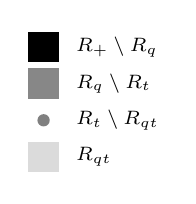
\begin{tikzpicture}[scale = .39]
\begin{scope}
\draw[draw = none, fill = black!100] (2,-1) rectangle (3,-2);
\node[anchor = west] at (3,-1.5) {\scriptsize  \  $R_+ \setminus R_q$};
\end{scope}
\begin{scope}[yshift = -34*1]
\draw[draw = none, fill = \mymidgray] (2,-1) rectangle (3,-2);
\node[anchor = west] at (3,-1.5) {\scriptsize  \  $R_q \setminus R_t$};
\end{scope}
\begin{scope}[yshift = -34*2]
\draw[thin, black!0] (2,-1) -- (3,-1);
\draw[thin, black!0] (2,-1) -- (2,-2);
\draw[thin, black!0] (2,-2) -- (3,-2);
\draw[thin, black!0] (3,-2) -- (3,-1);
\draw[draw = none, fill = gray!100] (2+0.5, -1-0.5) circle (.2);
\node[anchor = west] at (3,-1.5) {\scriptsize  \  $R_t \setminus R_{qt}$};
\end{scope}
\begin{scope}[yshift = -34*3]
\draw[draw = none, fill = black!14] (2,-1) rectangle (3,-2);
\node[anchor = west] at (3,-1.5) {\scriptsize \  $R_{qt}$};
\end{scope}
\end{tikzpicture}}
    \end{array}
  \]
\(s_\mu[-MX^{1,1}] \cdot 1 = \nabla s_\mu = \omega\pol_X H\) (up to
\(q,t\)-monomial)
\end{frame}
\begin{frame}{Dens and nests}
  \begin{theorem}[Blasiak-Haiman-Morse-Pun-S. (\(2021^+\))]
    For every partition \(\mu\) and coprime positive integers \(m,n\),
    we have 
    \begin{align*}
      & s_\mu[-MX^{m,n}] \cdot 1 \\ & = (-1)^{p(\mu)}
      (qt)^{p(\mu)+m \sum_{i=1}^h \binom{\gamma_i}{2}}\sum_\pi t^{\area(\pi)}
      q^{\dinv_p(\pi)} \omega \Gcal_{\nu(\pi)}(X;q^{-1})
    \end{align*}
  \end{theorem}
  \begin{itemize}
  \item Combinatorial RHS: Over all \emph{nests} \(\pi\) in a
    \emph{den} associated to \(\mu\) and \(m,n\).\pause
  \item Conjectured by Loehr-Warrington (2008) when \(n=1\) with different
    combinatorics (but bijectively related).
  \end{itemize}
\end{frame}
\begin{frame}{Dens and nests}
  \begin{theorem}[Blasiak-Haiman-Morse-Pun-S. (\(2021^+\))]
    For every partition \(\mu\) and coprime positive integers \(m,n\),
    we have 
    \begin{align*}
      & s_\mu[-MX^{m,n}] \cdot 1 \\ & = (-1)^{p(\mu)}
      (qt)^{p(\mu)+m \sum_{i=1}^h \binom{\gamma_i}{2}}\sum_\pi t^{\area(\pi)}
      q^{\dinv_p(\pi)} \omega \Gcal_{\nu(\pi)}(X;q^{-1})
    \end{align*}
  \end{theorem}
  \(\mu = \ydiagram{4,3,3}\)\pause
  \begin{itemize}
  \item \(p(\mu) = \) number of boxes with positive content. \(\ydiagram{4,3,3}*[*(blue)]{1+3,2+1}\) \pause
  \item \(h = m (\text{largest hook length in }\mu) =
    m(\mu_1+\ell(\mu)-1)\). \(\ydiagram{4,3,3}*[*(red)]{4,1,1}\)\pause
  \end{itemize}
\end{frame}
\begin{frame}{Dens and nests}
  \begin{theorem}[Blasiak-Haiman-Morse-Pun-S. (\(2021^+\))]
    For every partition \(\mu\) and coprime positive integers \(m,n\),
    we have 
    \begin{align*}
      & s_\mu[-MX^{m,n}] \cdot 1 \\ & = (-1)^{p(\mu)}
      (qt)^{p(\mu)+m \sum_{i=1}^h \binom{\gamma_i}{2}}\sum_\pi t^{\area(\pi)}
      q^{\dinv_p(\pi)} \omega \Gcal_{\nu(\pi)}(X;q^{-1})
    \end{align*}
  \end{theorem}
  \(\mu = \ydiagram{4,3,3}\)
  \begin{itemize}
  \item \(\gamma(\mu)\) is the tuple of the sizes of content diagonals.\pause 
  \item \(\mu=\ydiagram{4,3,3} \implies \gamma=(1,2,3,2,1,1)\).
  \end{itemize}
\end{frame}
\begin{frame}{Dens and nests}
  For given partition \(\lambda\)
  \begin{itemize}
  \item \(\delta_i(\lambda) = \chi(\lambda_1-1-i \text{ is the content
    of the last box of some row of }\lambda)\)  \pause
  \item \(\mu = \ytableaushort{{}{}{}3,{}{}1,{}{}0} \implies \delta(\mu) =
    (1,0,1,1,0,0,\ldots)\) \pause
  \item \(\epsilon_i(\lambda) = \chi(i \geq \lambda_1)\) \pause
  \item \(\mu = \ydiagram{4,3,3} \implies \epsilon(\mu) = (0,0,0,0,1,1,\ldots)\)
  \end{itemize}
\end{frame}
\begin{frame}{Dens and nests}
  To construct a (simplified) den, \pause
  \begin{enumerate}
  \item Draw the line connecting \((0,\frac{n}{m}h)\) and \((h,0)\)\pause
  \item Relationship between \(\delta\) and \(\epsilon\) tell us where to place a lattice point on each
    vertical, (weakly) below the line.\pause
  \item If \(\delta_i(\mu) > \epsilon_i(\mu)\), lattice point
    on \(x = im\) is a \emph{source}.\pause
  \item Similarly, \(\delta_i(\mu) < \epsilon_i(\mu)\implies\)  point
    on \(x=im\) is a \emph{sink}.\pause
  \end{enumerate}
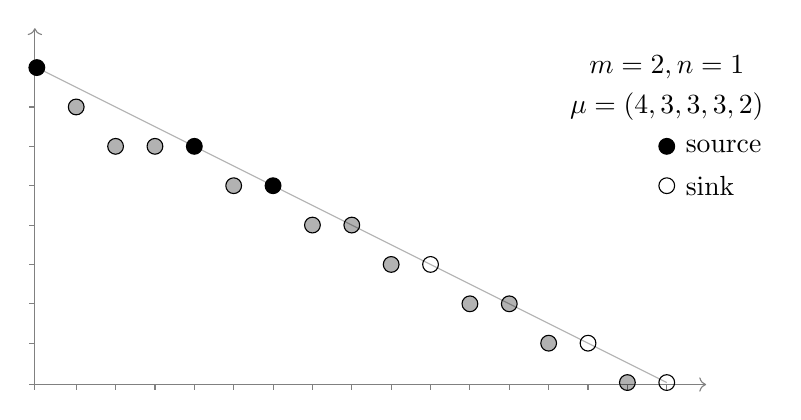
\begin{tikzpicture}[scale=.5]
% axes
\draw [->,gray] (-.05,-.05) -- (17,-.050);
\draw [->,gray] (-.05,-.05) -- (-.05,9);
\foreach \x in {-.05,1,2,3,4,5,6,7,8,9,10,11,12,13,14,15,16}
  \draw [gray] (\x ,-.050) -- (\x,-.2);
\foreach \y in {-.05,1,2,3,4,5,6,7,8}
  \draw [gray](-.05,\y) -- (-.2,\y);
% bounding line
\draw [black!30] (0,8) -- (16,0);
% heads and feet
\draw [fill] (0,8) circle (.2);
\draw [fill, fill opacity=.3] (1,7) circle (.2);
\draw [fill, fill opacity=.3] (2,6) circle (.2);
\draw [fill, fill opacity=.3] (3,6) circle (.2);
\draw [fill] (4,6) circle (.2);
\draw [fill, fill opacity=.3] (5,5) circle (.2);
\draw [fill] (6,5) circle (.2);
\draw [fill, fill opacity=.3] (7,4) circle (.2);
\draw [fill, fill opacity=.3] (8,4) circle (.2);
\draw [fill, fill opacity=.3] (9,3) circle (.2);
\draw (10,3) circle (.2);
\draw [fill, fill opacity=.3] (11,2) circle (.2);
\draw [fill, fill opacity=.3] (12,2) circle (.2);
\draw [fill, fill opacity=.3] (13,1) circle (.2);
\draw (14,1) circle (.2);
\draw [fill, fill opacity=.3] (15,0) circle (.2);
\draw (16,0) circle (.2);
%forbidden point
% \draw (2,7) node[very thick, cross=4pt] {};
% highest nest
%\draw (6,5) -- (6,4) -- (8,4) -- (8,3) -- (10,3);
%\draw [thick,dotted] (4,6) -- (4,5) -- (5,5) -- (5,4) -- (6,4) -- (6,3)
%-- (8,3) -- (8,2) -- (12,2) -- (12,1) -- (14,1);
%\draw  (.05,8) -- (.05,7) -- (1,7) -- (1,6) -- (3,6) -- (3,5)
% -- (4,5) -- (4,4) -- (5,4) -- (5,3) -- (6,3)
% --(6,2) -- (8,2) -- (8,1) -- (12,1) -- (12,.05) -- (16,.05);
\node at (16,8) {\(m=2, n=1\)};
\node at (16,7) {\(\mu = (4,3,3,3,2)\)};
\draw [fill] (16,6) circle (.2);
\node [right] at (16,6) {$\ \text{source}$};
\draw (16,5) circle (.2);
\node [right] at (16,5) {$\ \text{sink}$};
\end{tikzpicture}
\end{frame}
\begin{frame}{Dens and nests}
  \begin{itemize}
  \item Number the sources left to right and the sinks right to left.\pause
  \item A \emph{nest} is a collection of east end 
      lattice paths \((\pi^{(1)},\ldots,\pi^{(r)})\) that lie weakly below
      the marked lattice points.\pause
  \item Each \(\pi^{(i)}\) begins with a south step, starting at
    source \(i\), and ends with an
    east step into sink \(i\).\pause
  \item Each \(\pi^{(i)}\) is \emph{nested below} \(\pi^{(i+1)}\).\pause
    \begin{itemize}
    \item The interval of \(x\)-coordinates of \(\pi^{(i+1)}\) is
      contained in the interval of \(x\)-coordinates of \(\pi^{(i)}\).\pause
    \item Top of a south run of \(\pi^{(i+1)}\) strictly above the top of a
      south run of \(\pi^{(i)}\) on same vertical.\pause
    \item Bottom of a south run of \(\pi^{(i)}\) strictly below the bottom of a
      south run of \(\pi^{(i+1)}\) on same vertical.\pause
    \end{itemize}
  \end{itemize}
\begin{tikzpicture}[scale=.5,baseline=1cm]
\draw (0,4) -- (0,3) -- (.95,3) -- (.95,2) -- (2.95,2) -- (2.95, 0) -- (5,0);
\draw (1.05,4) -- (1.05,3) -- (3.05,3) -- (3.05,1) -- (4,1);
\node [below] at (1,1.8) {$\pi $};
\node [above] at (3.5,3) {$\pi '$};
\end{tikzpicture}
\end{frame}
\begin{frame}{Dens and nests}
  Example of the ``highest nest'' \(\pi^0\)
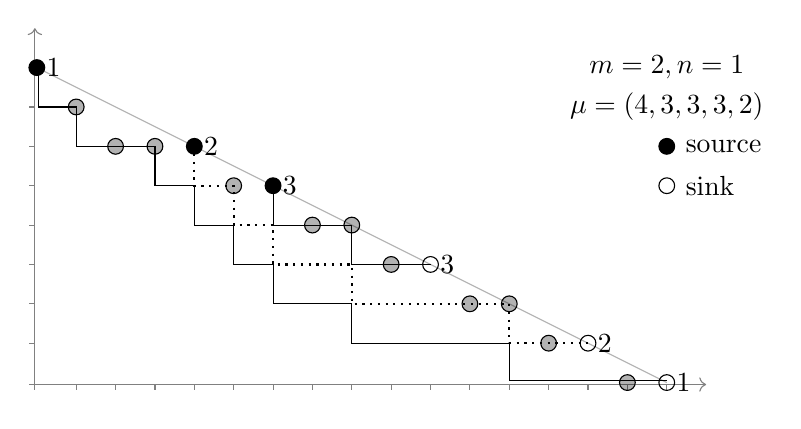
\begin{tikzpicture}[scale=.5]
% axes
\draw [->,gray] (-.05,-.05) -- (17,-.050);
\draw [->,gray] (-.05,-.05) -- (-.05,9);
\foreach \x in {-.05,1,2,3,4,5,6,7,8,9,10,11,12,13,14,15,16}
  \draw [gray] (\x ,-.050) -- (\x,-.2);
\foreach \y in {-.05,1,2,3,4,5,6,7,8}
  \draw [gray](-.05,\y) -- (-.2,\y);
% bounding line
\draw [black!30] (0,8) -- (16,0);
% heads and feet
\node [right] at (0,8) {1};
\node [right] at (4,6) {2};
\node [right] at (6,5) {3};
\node [right] at (10,3) {3};
\node [right] at (14,1) {2};
\node [right] at (16,0) {1};
\draw [fill] (0,8) circle (.2);
\draw [fill, fill opacity=.3] (1,7) circle (.2);
\draw [fill, fill opacity=.3] (2,6) circle (.2);
\draw [fill, fill opacity=.3] (3,6) circle (.2);
\draw [fill] (4,6) circle (.2);
\draw [fill, fill opacity=.3] (5,5) circle (.2);
\draw [fill] (6,5) circle (.2);
\draw [fill, fill opacity=.3] (7,4) circle (.2);
\draw [fill, fill opacity=.3] (8,4) circle (.2);
\draw [fill, fill opacity=.3] (9,3) circle (.2);
\draw (10,3) circle (.2);
\draw [fill, fill opacity=.3] (11,2) circle (.2);
\draw [fill, fill opacity=.3] (12,2) circle (.2);
\draw [fill, fill opacity=.3] (13,1) circle (.2);
\draw (14,1) circle (.2);
\draw [fill, fill opacity=.3] (15,0) circle (.2);
\draw (16,0) circle (.2);
%forbidden point
% \draw (2,7) node[very thick, cross=4pt] {};
% highest nest
\draw (6,5) -- (6,4) -- (8,4) -- (8,3) -- (10,3);
\draw [thick,dotted] (4,6) -- (4,5) -- (5,5) -- (5,4) -- (6,4) -- (6,3)
-- (8,3) -- (8,2) -- (12,2) -- (12,1) -- (14,1);
\draw  (.05,8) -- (.05,7) -- (1,7) -- (1,6) -- (3,6) -- (3,5)
 -- (4,5) -- (4,4) -- (5,4) -- (5,3) -- (6,3)
 --(6,2) -- (8,2) -- (8,1) -- (12,1) -- (12,.05) -- (16,.05);
\node at (16,8) {\(m=2, n=1\)};
\node at (16,7) {\(\mu = (4,3,3,3,2)\)};
\draw [fill] (16,6) circle (.2);
\node [right] at (16,6) {$\ \text{source}$};
\draw (16,5) circle (.2);
\node [right] at (16,5) {$\ \text{sink}$};
\end{tikzpicture}
\end{frame}
\begin{frame}{Dens and nests}
  Example of another nest. 
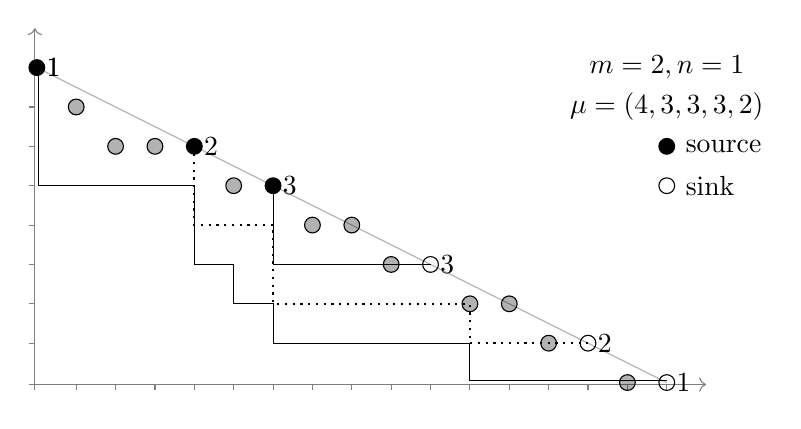
\begin{tikzpicture}[scale=.5]
% axes
\draw [->,gray] (-.05,-.05) -- (17,-.050);
\draw [->,gray] (-.05,-.05) -- (-.05,9);
\foreach \x in {-.05,1,2,3,4,5,6,7,8,9,10,11,12,13,14,15,16}
  \draw [gray] (\x ,-.050) -- (\x,-.2);
\foreach \y in {-.05,1,2,3,4,5,6,7,8}
  \draw [gray](-.05,\y) -- (-.2,\y);
% bounding line
\draw [black!30] (0,8) -- (16,0);
% heads and feet
\node [right] at (0,8) {1};
\node [right] at (4,6) {2};
\node [right] at (6,5) {3};
\node [right] at (10,3) {3};
\node [right] at (14,1) {2};
\node [right] at (16,0) {1};
\draw [fill] (0,8) circle (.2);
\node [right] at (0,8) {1};
\draw [fill, fill opacity=.3] (1,7) circle (.2);
\draw [fill, fill opacity=.3] (2,6) circle (.2);
\draw [fill, fill opacity=.3] (3,6) circle (.2);
\draw [fill] (4,6) circle (.2);
\draw [fill, fill opacity=.3] (5,5) circle (.2);
\draw [fill] (6,5) circle (.2);
\draw [fill, fill opacity=.3] (7,4) circle (.2);
\draw [fill, fill opacity=.3] (8,4) circle (.2);
\draw [fill, fill opacity=.3] (9,3) circle (.2);
\draw (10,3) circle (.2);
\draw [fill, fill opacity=.3] (11,2) circle (.2);
\draw [fill, fill opacity=.3] (12,2) circle (.2);
\draw [fill, fill opacity=.3] (13,1) circle (.2);
\draw (14,1) circle (.2);
\draw [fill, fill opacity=.3] (15,0) circle (.2);
\draw (16,0) circle (.2);
%forbidden point
% \draw (2,7) node[very thick, cross=4pt] {};
% highest nest
\draw (6,5) -- (6,3) -- (10,3);
\draw [thick,dotted] (4,6) -- (4,4) -- (6,4) -- (6,2)
-- (8,2) -- (11,2) -- (11,1) -- (14,1);
\draw  (.05,8) -- (.05,5) -- 
(4,5) -- (4,3) -- (5,3)
 --(5,2) -- (6,2) -- (6,1) --  (11,1) -- (11,.05) -- (16,.05);
\node at (16,8) {\(m=2, n=1\)};
\node at (16,7) {\(\mu = (4,3,3,3,2)\)};
\draw [fill] (16,6) circle (.2);
\node [right] at (16,6) {$\ \text{source}$};
\draw (16,5) circle (.2);
\node [right] at (16,5) {$\ \text{sink}$};
\end{tikzpicture}
\end{frame}
\begin{frame}{Area}
  \(\area(\pi) = \sum_{i=1}^r \area(\pi_{i})\) where
    \(\area(\pi_{i}) = \) number of lattice squares between
    \(\pi_{i}\) and \(\pi^0_{i}\).\pause

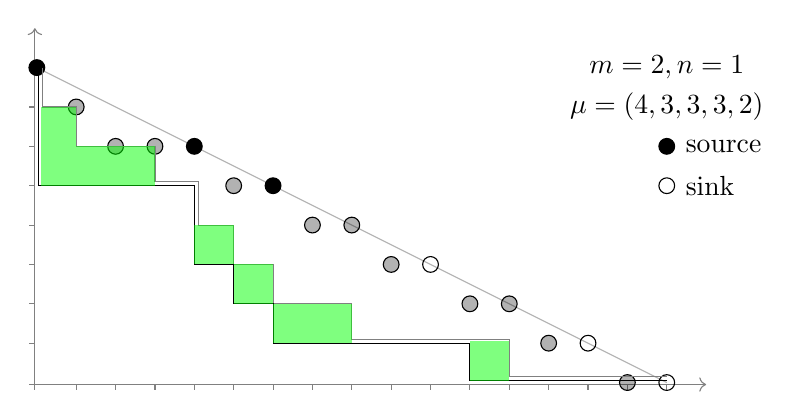
\begin{tikzpicture}[scale=.5]
% axes
\draw [->,gray] (-.05,-.05) -- (17,-.050);
\draw [->,gray] (-.05,-.05) -- (-.05,9);
\foreach \x in {-.05,1,2,3,4,5,6,7,8,9,10,11,12,13,14,15,16}
  \draw [gray] (\x ,-.050) -- (\x,-.2);
\foreach \y in {-.05,1,2,3,4,5,6,7,8}
  \draw [gray](-.05,\y) -- (-.2,\y);
% bounding line
\draw [black!30] (0,8) -- (16,0);
% heads and feet
\draw [fill] (0,8) circle (.2);
\draw [fill, fill opacity=.3] (1,7) circle (.2);
\draw [fill, fill opacity=.3] (2,6) circle (.2);
\draw [fill, fill opacity=.3] (3,6) circle (.2);
\draw [fill] (4,6) circle (.2);
\draw [fill, fill opacity=.3] (5,5) circle (.2);
\draw [fill] (6,5) circle (.2);
\draw [fill, fill opacity=.3] (7,4) circle (.2);
\draw [fill, fill opacity=.3] (8,4) circle (.2);
\draw [fill, fill opacity=.3] (9,3) circle (.2);
\draw (10,3) circle (.2);
\draw [fill, fill opacity=.3] (11,2) circle (.2);
\draw [fill, fill opacity=.3] (12,2) circle (.2);
\draw [fill, fill opacity=.3] (13,1) circle (.2);
\draw (14,1) circle (.2);
\draw [fill, fill opacity=.3] (15,0) circle (.2);
\draw (16,0) circle (.2);
%forbidden point
% \draw (2,7) node[very thick, cross=4pt] {};
% highest nest
\draw[gray]  (.15,8) -- (.15,7) -- (1,7) -- (1,6) -- (3,6) -- (3,5.1)
 -- (4.1,5.1) -- (4.1,4) -- (5,4) -- (5,3) -- (6,3)
 --(6,2) -- (8,2) -- (8,1.1) -- (12,1.1) -- (12,.15) -- (16,.15);
\draw  (.05,8) -- (.05,5) -- 
(4,5) -- (4,3) -- (5,3)
 --(5,2) -- (6,2) -- (6,1) --  (11,1) -- (11,.05) -- (16,.05);
\draw [draw=none, fill=green, fill opacity = .5] (.1,7) rectangle (1,6);
\draw [draw=none, fill=green, fill opacity = .5] (.1,6) rectangle (1,5);
\draw [draw=none, fill=green, fill opacity = .5] (1,6) rectangle (2,5);
\draw [draw=none, fill=green, fill opacity = .5] (2,6) rectangle (3,5);
\draw [draw=none, fill=green, fill opacity = .5] (4,4) rectangle (5,3);
\draw [draw=none, fill=green, fill opacity = .5] (5,3) rectangle (6,2);
\draw [draw=none, fill=green, fill opacity = .5] (6,2) rectangle (7,1);
\draw [draw=none, fill=green, fill opacity = .5] (7,2) rectangle (8,1);
\draw [draw=none, fill=green, fill opacity = .5] (11,1.05) rectangle (12,0.05);
\node at (16,8) {\(m=2, n=1\)};
\node at (16,7) {\(\mu = (4,3,3,3,2)\)};
\draw [fill] (16,6) circle (.2);
\node [right] at (16,6) {$\ \text{source}$};
\draw (16,5) circle (.2);
\node [right] at (16,5) {$\ \text{sink}$};
\end{tikzpicture}
\(\area(\pi_1) = 9\)
\end{frame}
\begin{frame}{Dens and nests}
  \begin{itemize}
  \item For \(p=\frac{n}{m}-\epsilon \in \R \setminus \Q\) and
    \(\epsilon\) small, \(\dinv_p(\pi) = \#\{(P,i,S,j)\}\) where\pause
    \begin{itemize}
    \item \(P\) is a non-sink lattice point in \(\pi_i\)
    \item \(S\) is a south step in \(\pi_j\)
    \item \(P\) is strictly to the left of \(S\)
    \item A line of slope \(-p\) passing through \(P\) passes through \(S\).
    \end{itemize}
  \end{itemize}\pause
  \[
\begin{array}{c}
\begin{tikzpicture}[scale=.5,]
\draw [thick] (3,-.2) -- (3,.8);
\node [right] at (3,.8) {$S$};
\draw [dashed] (-.5,2) -- (3.5,0);
\draw [fill] (0,1.75) circle (.1);
\node [below left] at (0,1.75) {$P$};
\end{tikzpicture}
\end{array}
\]
\end{frame}
\begin{frame}{dinv}
  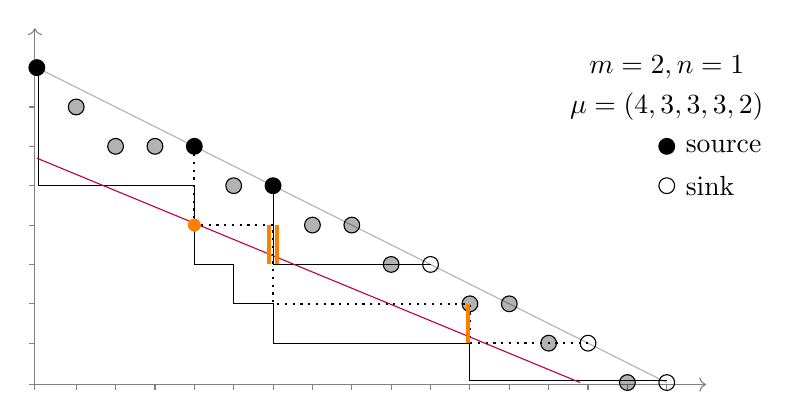
\begin{tikzpicture}[scale=.5]
% axes
\draw [->,gray] (-.05,-.05) -- (17,-.050);
\draw [->,gray] (-.05,-.05) -- (-.05,9);
\foreach \x in {-.05,1,2,3,4,5,6,7,8,9,10,11,12,13,14,15,16}
  \draw [gray] (\x ,-.050) -- (\x,-.2);
\foreach \y in {-.05,1,2,3,4,5,6,7,8}
  \draw [gray](-.05,\y) -- (-.2,\y);
% bounding line
\draw [black!30] (0,8) -- (16,0);
% heads and feet
\draw [fill] (0,8) circle (.2);
\draw [fill, fill opacity=.3] (1,7) circle (.2);
\draw [fill, fill opacity=.3] (2,6) circle (.2);
\draw [fill, fill opacity=.3] (3,6) circle (.2);
\draw [fill] (4,6) circle (.2);
\draw [fill, fill opacity=.3] (5,5) circle (.2);
\draw [fill] (6,5) circle (.2);
\draw [fill, fill opacity=.3] (7,4) circle (.2);
\draw [fill, fill opacity=.3] (8,4) circle (.2);
\draw [fill, fill opacity=.3] (9,3) circle (.2);
\draw (10,3) circle (.2);
\draw [fill, fill opacity=.3] (11,2) circle (.2);
\draw [fill, fill opacity=.3] (12,2) circle (.2);
\draw [fill, fill opacity=.3] (13,1) circle (.2);
\draw (14,1) circle (.2);
\draw [fill, fill opacity=.3] (15,0) circle (.2);
\draw (16,0) circle (.2);
%forbidden point
% \draw (2,7) node[very thick, cross=4pt] {};
% highest nest
\draw (6,5) -- (6,3) -- (10,3);
\draw [thick,dotted] (4,6) -- (4,4) -- (6,4) -- (6,2)
-- (8,2) -- (11,2) -- (11,1) -- (14,1);
\draw  (.05,8) -- (.05,5) -- 
(4,5) -- (4,3) -- (5,3)
 --(5,2) -- (6,2) -- (6,1) --  (11,1) -- (11,.05) -- (16,.05);
\draw[purple] (0,5.7) -- (13.8,0);
\draw[fill, orange] (4,4) circle (.15);
\draw[very thick, orange, visible on=<2->] (6.1,3) -- (6.1,4);
\draw[very thick, orange, visible on=<3->] (5.90,3) -- (5.90,4);
\draw[very thick, orange, visible on=<4->] (10.95,1) -- (10.95,2);
\node at (16,8) {\(m=2, n=1\)};
\node at (16,7) {\(\mu = (4,3,3,3,2)\)};
\draw [fill] (16,6) circle (.2);
\node [right] at (16,6) {$\ \text{source}$};
\draw (16,5) circle (.2);
\node [right] at (16,5) {$\ \text{sink}$};
\end{tikzpicture}

Contributes 3 to the dinv.
\end{frame}
\begin{frame}{Associating a tuple of skew partitions to a nest}
  \begin{itemize}
  \item Each vertical line \(x=i\) will give a skew partition.\pause
  \item South steps of each path will contribute a row.\pause
  \item Content determined by how far down south step is from highest
    lattice point under the line + \(j\) for \(\pi_j\).\pause
  \item Tuple ordered by how far marked lattice points are from slight
    perturbation of line.\pause
  \end{itemize}
  \[
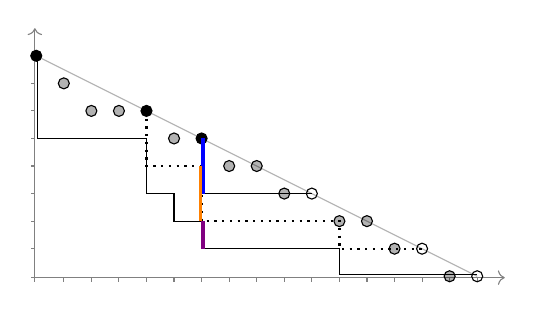
\begin{tikzpicture}[scale=.35]
% axes
\draw [->,gray] (-.05,-.05) -- (17,-.050);
\draw [->,gray] (-.05,-.05) -- (-.05,9);
\foreach \x in {-.05,1,2,3,4,5,6,7,8,9,10,11,12,13,14,15,16}
  \draw [gray] (\x ,-.050) -- (\x,-.2);
\foreach \y in {-.05,1,2,3,4,5,6,7,8}
  \draw [gray](-.05,\y) -- (-.2,\y);
% bounding line
\draw [black!30] (0,8) -- (16,0);
% heads and feet
\draw [fill] (0,8) circle (.2);
\draw [fill, fill opacity=.3] (1,7) circle (.2);
\draw [fill, fill opacity=.3] (2,6) circle (.2);
\draw [fill, fill opacity=.3] (3,6) circle (.2);
\draw [fill] (4,6) circle (.2);
\draw [fill, fill opacity=.3] (5,5) circle (.2);
\draw [fill] (6,5) circle (.2);
\draw [fill, fill opacity=.3] (7,4) circle (.2);
\draw [fill, fill opacity=.3] (8,4) circle (.2);
\draw [fill, fill opacity=.3] (9,3) circle (.2);
\draw (10,3) circle (.2);
\draw [fill, fill opacity=.3] (11,2) circle (.2);
\draw [fill, fill opacity=.3] (12,2) circle (.2);
\draw [fill, fill opacity=.3] (13,1) circle (.2);
\draw (14,1) circle (.2);
\draw [fill, fill opacity=.3] (15,0) circle (.2);
\draw (16,0) circle (.2);
%forbidden point
% \draw (2,7) node[very thick, cross=4pt] {};
% highest nest
\draw (6,5) -- (6,3) -- (10,3);
\draw [thick,dotted] (4,6) -- (4,4) -- (6,4) -- (6,2)
-- (8,2) -- (11,2) -- (11,1) -- (14,1);
\draw  (.05,8) -- (.05,5) -- 
(4,5) -- (4,3) -- (5,3)
 --(5,2) -- (6,2) -- (6,1) --  (11,1) -- (11,.05) -- (16,.05);
\draw[very thick, blue, visible on = <8->] (6.05,3) -- (6.05,5);
\draw[very thick, orange, visible on = <7->] (5.95,2) -- (5.95,4);
\draw[very thick, violet, visible on = <6->] (6.05,1) -- (6.05,2);
\end{tikzpicture}
  \]\pause
  \[
      \begin{ytableau}
        \none[\cdot] & \none[\cdot] & \none[\cdot] & \none[\cdot] &
        *(violet) \\
        \none[\cdot] & \none[\cdot] & \none[\cdot] & *(orange) &
        *(orange) \\
        \none[\cdot] & \none[\cdot] & \none[\cdot] & *(blue) & *(blue)
      \end{ytableau}
  \]

\end{frame}
\begin{frame}{Dens and nests}
  \begin{itemize}
  \item In our paper, we provide a more general definition of den as a
    tuple of data \((h,p,d,e) \in \Z_{>0} \times (\R \setminus \Q)
    \times \Z^{h+1} \times \Z^{h+1}\) subject to some conditions.\pause 
  \item To each den we can
    associate a tame Catalanimal \(H\) and give a corresponding
    shuffle theorem as a sum over the nests of the den.\pause
  \item These results hold ``stably.'' In other words, a stronger result is
    proven before applying polynomial truncation.\pause
  \item This allows us to simultaneously generalize the
    \(s_\lambda[-MX^{m,n}]\) formula and our ``shuffle theorem for
    paths under any line'' formula (BHMPS).
  \end{itemize}
\end{frame}
\begin{frame}{Other exhibits for next time}
  \begin{itemize}
  \item For each LLT polynomial \(\Gcal_\nu\) and coprime \((m,n)\) with \(m > 0\), an
    \(m,n\)-cuddly Catalanimal with cub \(\Gcal_\nu\) is given. (BHMPS)\pause
  \item Special cases include Schur functions and Hall-Littlewood
    polynomials.\pause
  \item Unicorn Catalanimals (or Catalan functions) where
    \(R_t = R_{qt} = \emptyset\) also have a rich
    (older) results and combinatorics, but served as
    inspiration. (Chen-Haiman, Blasiak-Morse-Pun-Summers, Blasiak-Morse-Pun)
  \end{itemize}
\end{frame}
\begin{frame}{Future work: exit through the gift shop}
  \begin{itemize}
  \item Is there a representation-theoretic model for \(\nabla
    s_\mu\)? For any Catalanimal associated to a den?\pause
  \item Any direct combinatorial formula (even a conjecture) for the Schur-expansion coefficients?\pause
  \item What other families of symmetric functions can be represented
    by Catalanimals? \pause Upcoming: Macdonald polynomials\pause
  \item What connections do Catalanimals have with machinery used to
    prove other shuffle theorems, such as work by Carlsson-Mellit?
  \end{itemize}
\end{frame}
\begin{frame}[shrink=10]
  \frametitle{Thank you for visiting!}
  \begin{bibdiv}
    \begin{biblist}
\bib{MR3556418}{article}{
   author={Bergeron, Francois},
   author={Garsia, Adriano},
   author={Sergel Leven, Emily},
   author={Xin, Guoce},
   title={Compositional $(km,kn)$-shuffle conjectures},
   journal={Int. Math. Res. Not. IMRN},
   date={2016},
   number={14},
   pages={4229--4270},
   issn={1073-7928},
   review={\MR{3556418}},
   doi={10.1093/imrn/rnv272},
}
\bib{paths}{article}{
  author={Blasiak, Jonah},
  author={Haiman, Mark},
  author={Morse, Jennifer},
  author={Pun, Anna},
  author={Seelinger, George H.},
  title={A Shuffle Theorem for Paths Under Any Line},
  year={2021},
  journal = {arXiv e-prints},
  eprint={arXiv:2102.07931}
}
\bib{delta}{article}{
  author={Blasiak, Jonah},
  author={Haiman, Mark},
  author={Morse, Jennifer},
  author={Pun, Anna},
  author={Seelinger, George H.},
  title={Dens, nests and the Loehr-Warrington conjecture},
  year={2021},
  journal = {arXiv e-prints},
  eprint={arXiv:2112.07070}
}
\bib{delta}{article}{
  author={Blasiak, Jonah},
  author={Haiman, Mark},
  author={Morse, Jennifer},
  author={Pun, Anna},
  author={Seelinger, George H.},
  title={LLT polynomials in the Schiffmann algebra},
  year={2021},
  journal = {arXiv e-prints},
  eprint={arXiv:2112.07063}
}
\bib{MR2922373}{article}{
   author={Burban, Igor},
   author={Schiffmann, Olivier},
   title={On the Hall algebra of an elliptic curve, I},
   journal={Duke Math. J.},
   volume={161},
   date={2012},
   number={7},
   pages={1171--1231},
   issn={0012-7094},
   review={\MR{2922373}},
   doi={10.1215/00127094-1593263},
}
\bib{MR3787405}{article}{
   author={Carlsson, Erik},
   author={Mellit, Anton},
   title={A proof of the shuffle conjecture},
   journal={J. Amer. Math. Soc.},
   volume={31},
   date={2018},
   number={3},
   pages={661--697},
   issn={0894-0347},
   review={\MR{3787405}},
   doi={10.1090/jams/893},
}
\bib{MR1214091}{article}{
   author={Garsia, Adriano M.},
   author={Haiman, Mark},
   title={A graded representation model for Macdonald's polynomials},
   journal={Proc. Nat. Acad. Sci. U.S.A.},
   volume={90},
   date={1993},
   number={8},
   pages={3607--3610},
   issn={0027-8424},
   review={\MR{1214091}},
   doi={10.1073/pnas.90.8.3607},
}
    \end{biblist}
  \end{bibdiv}
\end{frame}
\begin{frame}[shrink=10]
  \frametitle{References continued}
  \begin{bibdiv}
    \begin{biblist}
\bib{GrojHai07}{article}{
  author={Grojnowski, Ian},
  author={Haiman, Mark},
  title={Affine Hecke algebras and positivity of LLT and Macdonald polynomials},
  year={2007},
  journal={Unpublished manuscript}
}
\bib{MR2115257}{article}{
    AUTHOR = {Haglund, J. and Haiman, M. and Loehr, N. and Remmel, J. B. and
              Ulyanov, A.},
     TITLE = {A combinatorial formula for the character of the diagonal
              coinvariants},
   JOURNAL = {Duke Math. J.},
  FJOURNAL = {Duke Mathematical Journal},
    VOLUME = {126},
      YEAR = {2005},
    NUMBER = {2},
     PAGES = {195--232},
      ISSN = {0012-7094},
   MRCLASS = {05E10 (05A30 20C30)},
  MRNUMBER = {2115257},
MRREVIEWER = {Edward E. Allen},
       DOI = {10.1215/S0012-7094-04-12621-1},
       URL = {https://doi-org.proxy01.its.virginia.edu/10.1215/S0012-7094-04-12621-1},
}
\bib{MR1839919}{article}{
   author={Haiman, Mark},
   title={Hilbert schemes, polygraphs and the Macdonald positivity
   conjecture},
   journal={J. Amer. Math. Soc.},
   volume={14},
   date={2001},
   number={4},
   pages={941--1006},
   issn={0894-0347},
   review={\MR{1839919}},
   doi={10.1090/S0894-0347-01-00373-3},
}
\bib{MR1918676}{article}{
   author={Haiman, Mark},
   title={Vanishing theorems and character formulas for the Hilbert scheme
   of points in the plane},
   journal={Invent. Math.},
   volume={149},
   date={2002},
   number={2},
   pages={371--407},
   issn={0020-9910},
   review={\MR{1918676}},
   doi={10.1007/s002220200219},
}
\bib{MR1399754}{article}{
   author={Lascoux, Alain},
   author={Leclerc, Bernard},
   author={Thibon, Jean-Yves},
   title={Ribbon tableaux, Hall-Littlewood functions and unipotent
   varieties},
   journal={S\'{e}m. Lothar. Combin.},
   volume={34},
   date={1995},
   pages={Art. B34g, approx. 23},
   review={\MR{1399754}},
}
\bib{MR2418288}{article}{
   author={Loehr, Nicholas A.},
   author={Warrington, Gregory S.},
   title={Nested quantum Dyck paths and $\nabla(s_\lambda)$},
   journal={Int. Math. Res. Not. IMRN},
   date={2008},
   number={5},
   pages={Art. ID rnm 157, 29},
   issn={1073-7928},
   review={\MR{2418288}},
   doi={10.1093/imrn/rnm157},
}
\bib{mellit}{article}{
       author = {{Mellit}, Anton},
        title = {Toric braids and $(m,n)$-parking functions},
      journal = {arXiv e-prints},
     keywords = {Mathematics - Combinatorics, Mathematics - Quantum Algebra, Mathematics - Representation Theory},
         year = {2016},
        month = {apr},
          eid = {arXiv:1604.07456},
        pages = {arXiv:1604.07456},
archivePrefix = {arXiv},
       eprint = {arXiv:1604.07456},
 primaryClass = {math.CO},
}
\bib{MR3283004}{article}{
   author={Negut, Andrei},
   title={The shuffle algebra revisited},
   journal={Int. Math. Res. Not. IMRN},
   date={2014},
   number={22},
   pages={6242--6275},
   issn={1073-7928},
   review={\MR{3283004}},
   doi={10.1093/imrn/rnt156},
}
    \end{biblist}
  \end{bibdiv}
\end{frame}

% \begin{frame}{Schiffmann Algebra}
%   \begin{itemize}
%   \item The operator \(e_k[-MX^{m,n}]\) corresponds to an action of
%     the “Schiffmann algebra'' \(\Ecal\) acting on \(\Lambda\).
%   \item For each \(m,n\) coprime, \(\Ecal\) has a subalgebra
%     isomorphic to \(\Lambda\), which we denote \(\Lambda[X^{m,n}]\),
%     and many relations between them.
%   \item 
%   \end{itemize}
% \end{frame}
% \begin{frame}
%   \frametitle{Any Line}
%   \begin{block}{Negut Elements}
%     For \(\bb \in \Z^l\), special elements \(D_\bb \in
%     \Ecal\) generalizing \(e_k[-MX^{m,n}]\).
%   \end{block}
%   \pause
%   \begin{block}{Theorem (Blasiak-Haiman-Morse-Pun-S., 2021a)}
%     Given \(r,s \in \R_{>0}\) such that \(p = s/r\) irrational, take
%     \((b_1,\ldots,b_l) \in \Z^l\) to be the south step sequence of highest path
%     \(\delta\) under the line \(y+px=s\).
%     \pause \[
%       D_{(b_1,\ldots,b_l)} \cdot 1 \pause =
%       \onslide<4->{\sum_{\lambda}}\onslide<5->
%       {
%         t^{\area(\lambda)}
%         q^{\dinv_p(\lambda)}}\onslide<4->{\omega \Gcal_{\nu(\lambda)}(X;q^{-1})}
%     \]
%     \onslide<4->{where summation is over all lattice paths under the line \(y+px=s\),}
%   \end{block}\pause
%   \begin{columns}
%     \begin{column}{0.2\textwidth}
%       \begin{tikzpicture}[scale=.25, baseline=-.5cm]
%         \draw[help lines] (0,0) grid (7.2,9.5); \draw [thick]
%         (0,9.2727) -- (6.8,0); \draw [very thick] (0,9) -- (0,6) --
%         (2,6) -- (2,3) -- (3,3) -- (3,1) -- (5,1) -- (5,0) -- (6,0);
%       \end{tikzpicture}
%     \end{column}
%     \begin{column}{0.8\textwidth}
%       \(\area(\lambda)\) as before\\
%       \(\dinv_p(\lambda) = \# p\)-balanced hooks \(\frac{\ell}{a+1} < p <
%       \frac{\ell+1}{a}\)\\
%     \end{column}
%   \end{columns}
% \end{frame}
% \begin{frame}{Key insight: Catalanimals}
% \(D_{(b_1,\ldots,b_l)} \cdot 1 = \pol_X \sigma x_1^{b_1} \cdots x_l^{b_l}\left( \frac{\prod_{i <
%       j+1} (1-q\,t\, z_i/z_j)}{\prod_{i<j} (1-q\,z_i/z_j)(1-t\,z_i/z_j)} \right)\)  
% \begin{itemize}
% \item \(\sigma \from \Q(q,t)[z][[z]] \to \) sends \(z^\alpha
%   \mapsto \chi_\alpha = \pm \chi_\lambda\) or 0.
% \item \(\pol_X\) sends \(\chi_\lambda \mapsto s_\lambda\) if
%   \(\lambda_l \geq 0\) and 0 otherwise.
% \end{itemize}
% \begin{definition}
%   A \emph{Catalanimal}  
% \end{definition}
% \end{frame}
\end{document}
%%% Local Variables:
%%% mode: latex
%%% TeX-master: t
%%% End:
